\documentclass{beamer}
\usepackage{multicol}

\usepackage{clrscode3e}
\usepackage{amsmath,amsfonts}
\usepackage{graphicx,color}

\newcommand{\bi}{\begin{itemize}}
\newcommand{\ii}{\item}
\newcommand{\ei}{\end{itemize}}
\newcommand{\bn}{\begin{enumerate}}
\newcommand{\en}{\end{enumerate}}
\newcommand{\set}[1]{\ensuremath{\left\{#1\right\}}}
\newcommand{\pr}[1]{\ensuremath{\mbox{Pr}\left\{#1\right\}}}
\newcommand{\flr}[1]{\ensuremath{\left\lfloor#1\right\rfloor}}
\newcommand{\ceil}[1]{\ensuremath{\left\lceil#1\right\rceil}}

\newcommand{\sect}[1]{
\section{#1}
\begin{frame}[fragile]\frametitle{#1}
}


\setlength{\tabcolsep}{4\tabcolsep}

\newcommand{\nop}[1]{}

\newcommand{\att}[2]{\attrib{#1}{#2}}
\newcommand{\attt}[3]{\attrib{\attrib{#1}{#2}}{#3}}
\newcommand{\atttt}[4]{\attrib{\attrib{\attrib{#1}{#2}}{#3}}{#4}}


\title{Notes on Red-black Trees}
\author{Geoffrey Matthews}
\begin{document}
\begin{frame}
  \maketitle
\end{frame}


\sect{Red-black trees}
\bi
\ii A variation of binary search trees.
\ii \textbf{Balanced:} height is $O(\lg n)$, where $n$ is number of nodes.
\ii Operations will take $O(\lg n)$ in worst case.
\ei

\end{frame}

\sect{Red-black trees}
\bi
\ii A \textbf{red-black tree} is a binary search tree.
\ii One bit per node stores an attribute \textit{color}, red or black.
\ii All leaves are empty (nil) and colored black.
\ii We use a sentinel $\attrib{T}{nil}$ for all the leaves of a
red-black tree $T$.
\ii $\attrib{\attrib{T}{nil}}{color}$ is black.
\ii The root's parent is also $\attrib{T}{nil}$.
\ii All other attributes ({\em key, left, right, p}) are inherited.
\ii We don't care about $\attrib{\attrib{T}{nil}}{key}$
\ei


\end{frame}

\sect{Red-black tree properties \hspace{3cm} (remember!)}

\begin{enumerate}
  \ii Every node is either red or black.
  \ii The root is black.
  \ii Every leaf ($\attrib{T}{nil}$) is black.
  \ii If a node is red, then both its children are black.
  \ii All paths from a node to descendent leaves
  have same number of black nodes, called {\bf black height}.
\end{enumerate}
\vfill
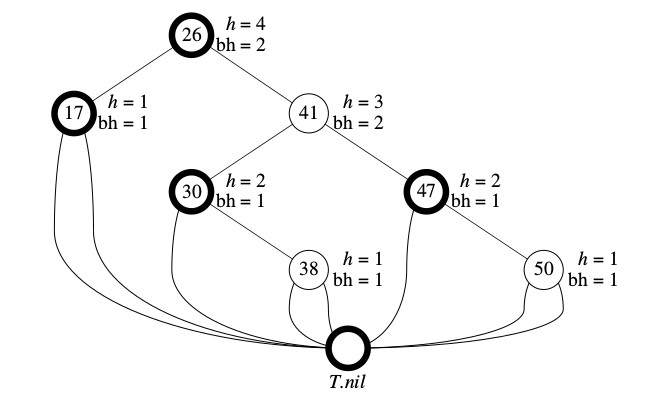
\includegraphics[scale=0.5]{example}
\end{frame}

\sect{Red-black tree}

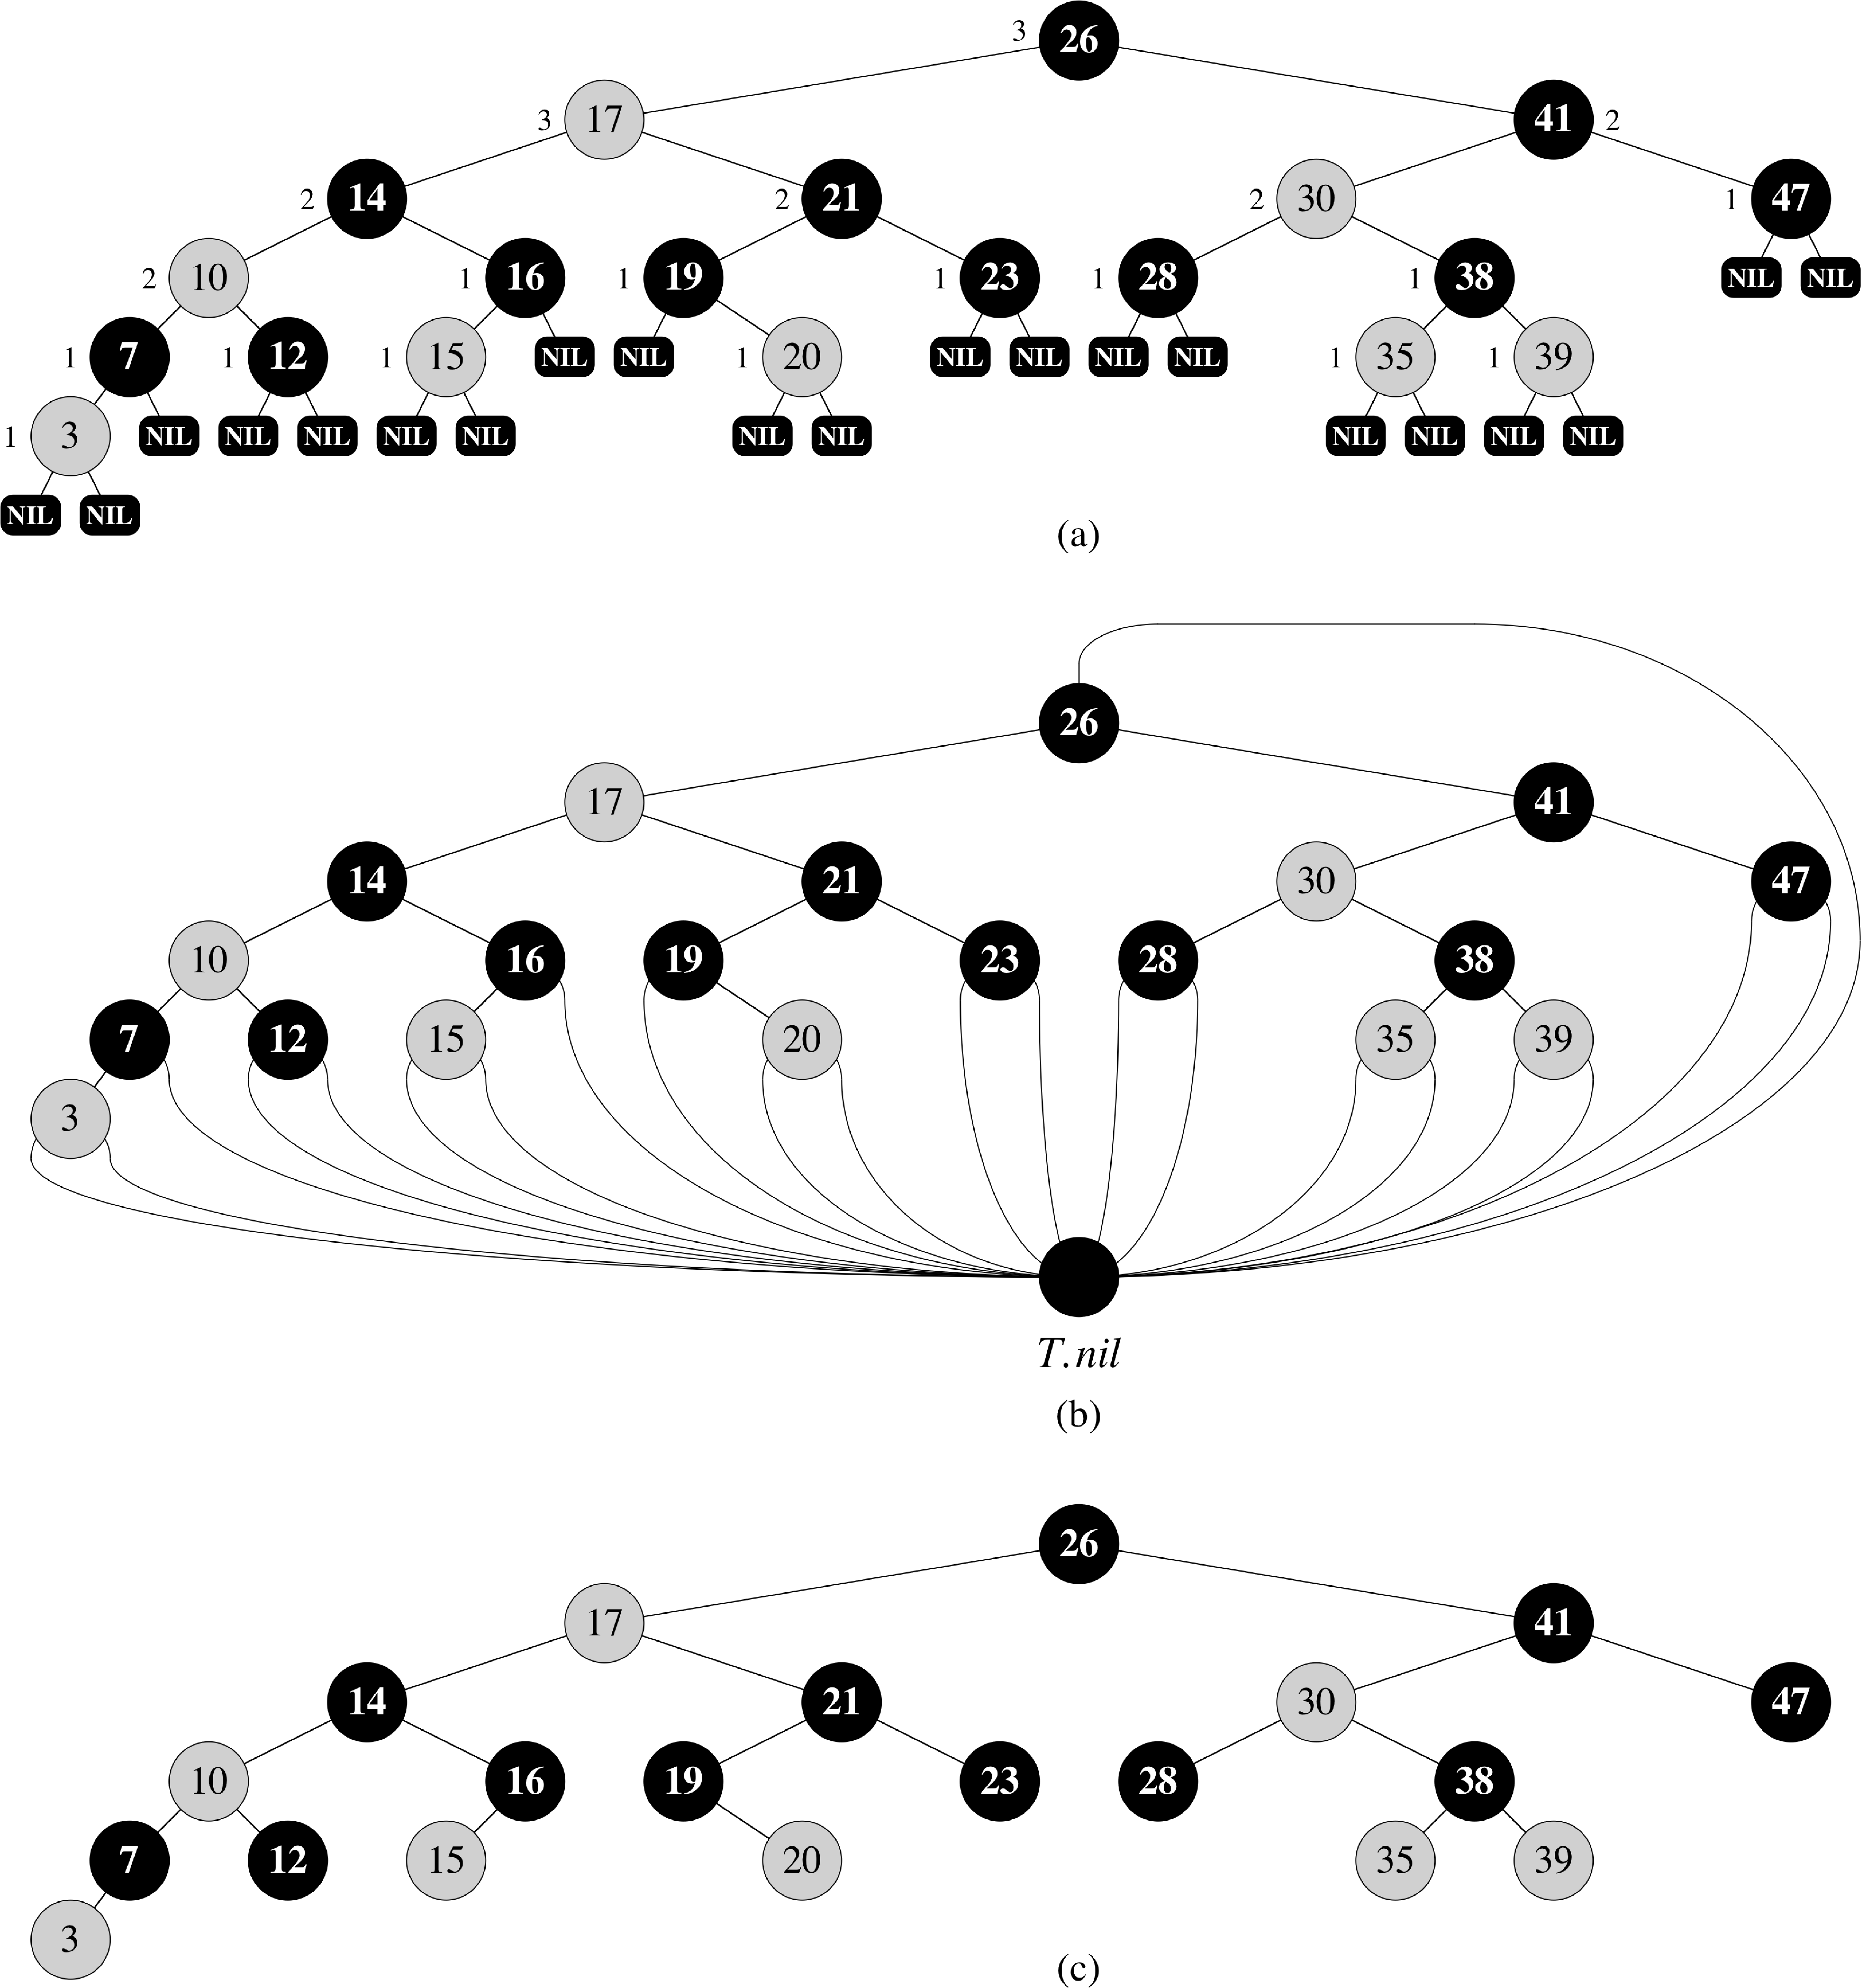
\includegraphics[height=0.8\textheight]{Fig-13-1.pdf}

\end{frame}

\sect{Height of a red-black tree} \bi \ii \textbf{Height of a node} is
the number of edges in longest path to leaf.  \ii
\textbf{Black-height} of a node $x$: bh($x$) is the number of black
nodes (including $\attrib{T}{nil}$) on a path from $x$ to a leaf, not
counting $x$.  \bi \ii By property 5, black-height is well defined.
\ii Changing the color of a node does not change its black-height.
\ii Changing the color of a node will change the black-height of its
ancestors.  \ei

\ei

\end{frame}

\sect{Claim 1:} Any node with height $h$ has black-height $\geq h/2$.

\bigskip

  \textbf{Proof}
\bi\ii
  By property 4, $\leq h/2$ nodes on the path from node to a leaf are
  red.\ii  Hence $\geq h/2$ are black.\ei

\end{frame}

\sect{Claim 2:} The subtree rooted at $x$ contains $\geq
  2^{\id{bh}(x)}   - 1$ internal nodes.

\bigskip
  
\textbf{Proof.}  By induction on height of $x$.

\textbf{Basis:} Height of $x=0\Rightarrow x$ is a leaf and so
$\id{bh}(x)=0$, $2^0-1=0$.

\textbf{Inductive step:}
\bi
\ii Let the height of $x$ be $h$.
\ii Any child of $x$ has height $h-1$ and black-height
either $bh(x)$ (if the child is red) or $bh(x)-1$ (if the child is black).
\ii By
inductive hypothesis, each child has $\geq 2^{\id{bh}(x)-1}-1$
internal nodes. \ii
Thus, the subtree rooted at $x$ contains $\geq 2\cdot
(2^{\id{bh}(x)-1}-1) + 1 = 2^{\id{bh}(x)}-1$ internal nodes.
\ei  

\end{frame}

\sect{Lemma:} A red-black tree with $n$ internal nodes
and height $h$ has
  \[
  h\leq 2\lg (n+1)\]

\bi\ii Recall proven claims:
\bi
\ii  Any node with height $h$ has black-height $\geq h/2$.
\ii  The subtree rooted at any node $x$ contains $\geq
  2^{\id{bh}(x)}   - 1$ internal nodes.
\ei\ei

\textbf{Proof}

 Let $h$ and $b$ be the height and black-height of the root,
 respectively.
 
 By the above two claims,
\[ n \geq 2^b-1 \geq 2^{h/2} - 1 \]
Adding 1 to both sides and then taking logs gives
\[ \lg(n+1) \geq h/2\]
which implies that
\[
h \leq 2\lg(n+1)
\]


\end{frame}

\sect{Operations on red-black trees}
\bi
\ii $\proc{Minimum}$, $\proc{Maximum}$, $\proc{Successor}$,
$\proc{Predecessor}$ and $\proc{Search}$ all run in $O(h) = O(\lg n)$
time.
\ii $\proc{Insert}$, what color to make the new node?
\bi \ii Red?
\bi\ii Might violate property 4.\ei
\ii Black?
\bi\ii Might violate property 5.\ei
\ei
\ii $\proc{Delete}$, what color was the old node?
\bi
\ii Red?
\bi\ii Successor might be black.\ei
\ii Black?
\bi\ii Could cause two reds in a row, and violate properties 2 and 5.\ei
\ei
\ei

\end{frame}

\sect{Rotations}

\bi
\ii Only pointers are changed.
\ii Won't upset binary-search-tree property.
\ii Doesn't care about red-black.
\ei

\begin{multicols}{2}
\begin{codebox}
  \Procname{$\proc{Left-Rotate}(T,x)$}
  \li $y \gets \attrib{x}{right}$
  \li $\attrib{x}{right} \gets \attrib{y}{left}$
  \li \If $\attrib{y}{left}\not = \attrib{T}{nil}$ \Do
  \li $\attrib{\attrib{y}{left}}{p} \gets x$ \End
  \li $\attrib{y}{p} \gets \attrib{x}{p}$
  \li \If $\attrib{x}{p} \isequal \attrib{T}{nil}$ \Do
  \li  $\attrib{T}{root} \gets y$ 
  \li \ElseIf $x \isequal \attrib{\attrib{x}{p}}{left}$ \Do
  \li $\attrib{\attrib{x}{p}}{left} \gets y$
  \li \Else $\attrib{\attrib{x}{p}}{right} \gets y$ \End
  \li $\attrib{y}{left} \gets x$
  \li $\attrib{x}{p} \gets y$
\end{codebox}
\columnbreak
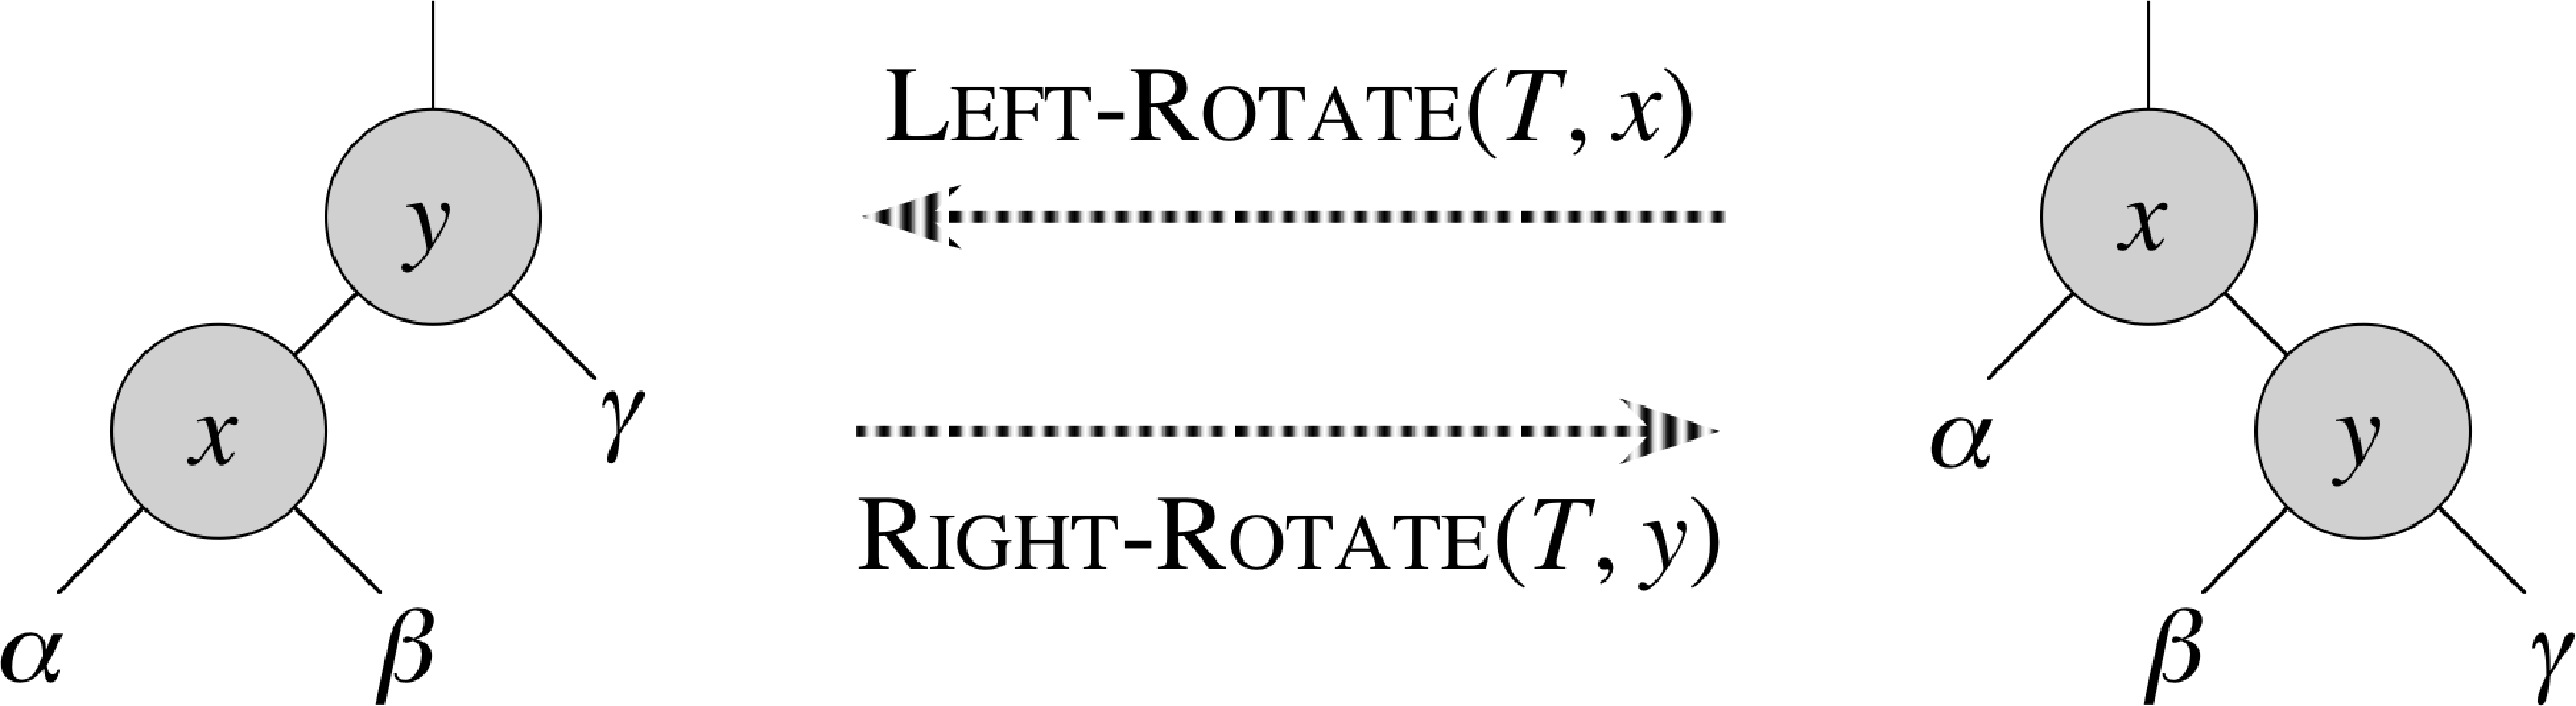
\includegraphics[width=0.5\textwidth]{Fig-13-2.pdf}

\vfill


 Assumes
\bi
\ii $\attrib{x}{right}\not = \attrib{T}{nil}$
\ii root's parent is $\attrib{T}{nil}$
\ei

\[\Theta(1)\]

\end{multicols}

\end{frame}
\sect{Rotations}

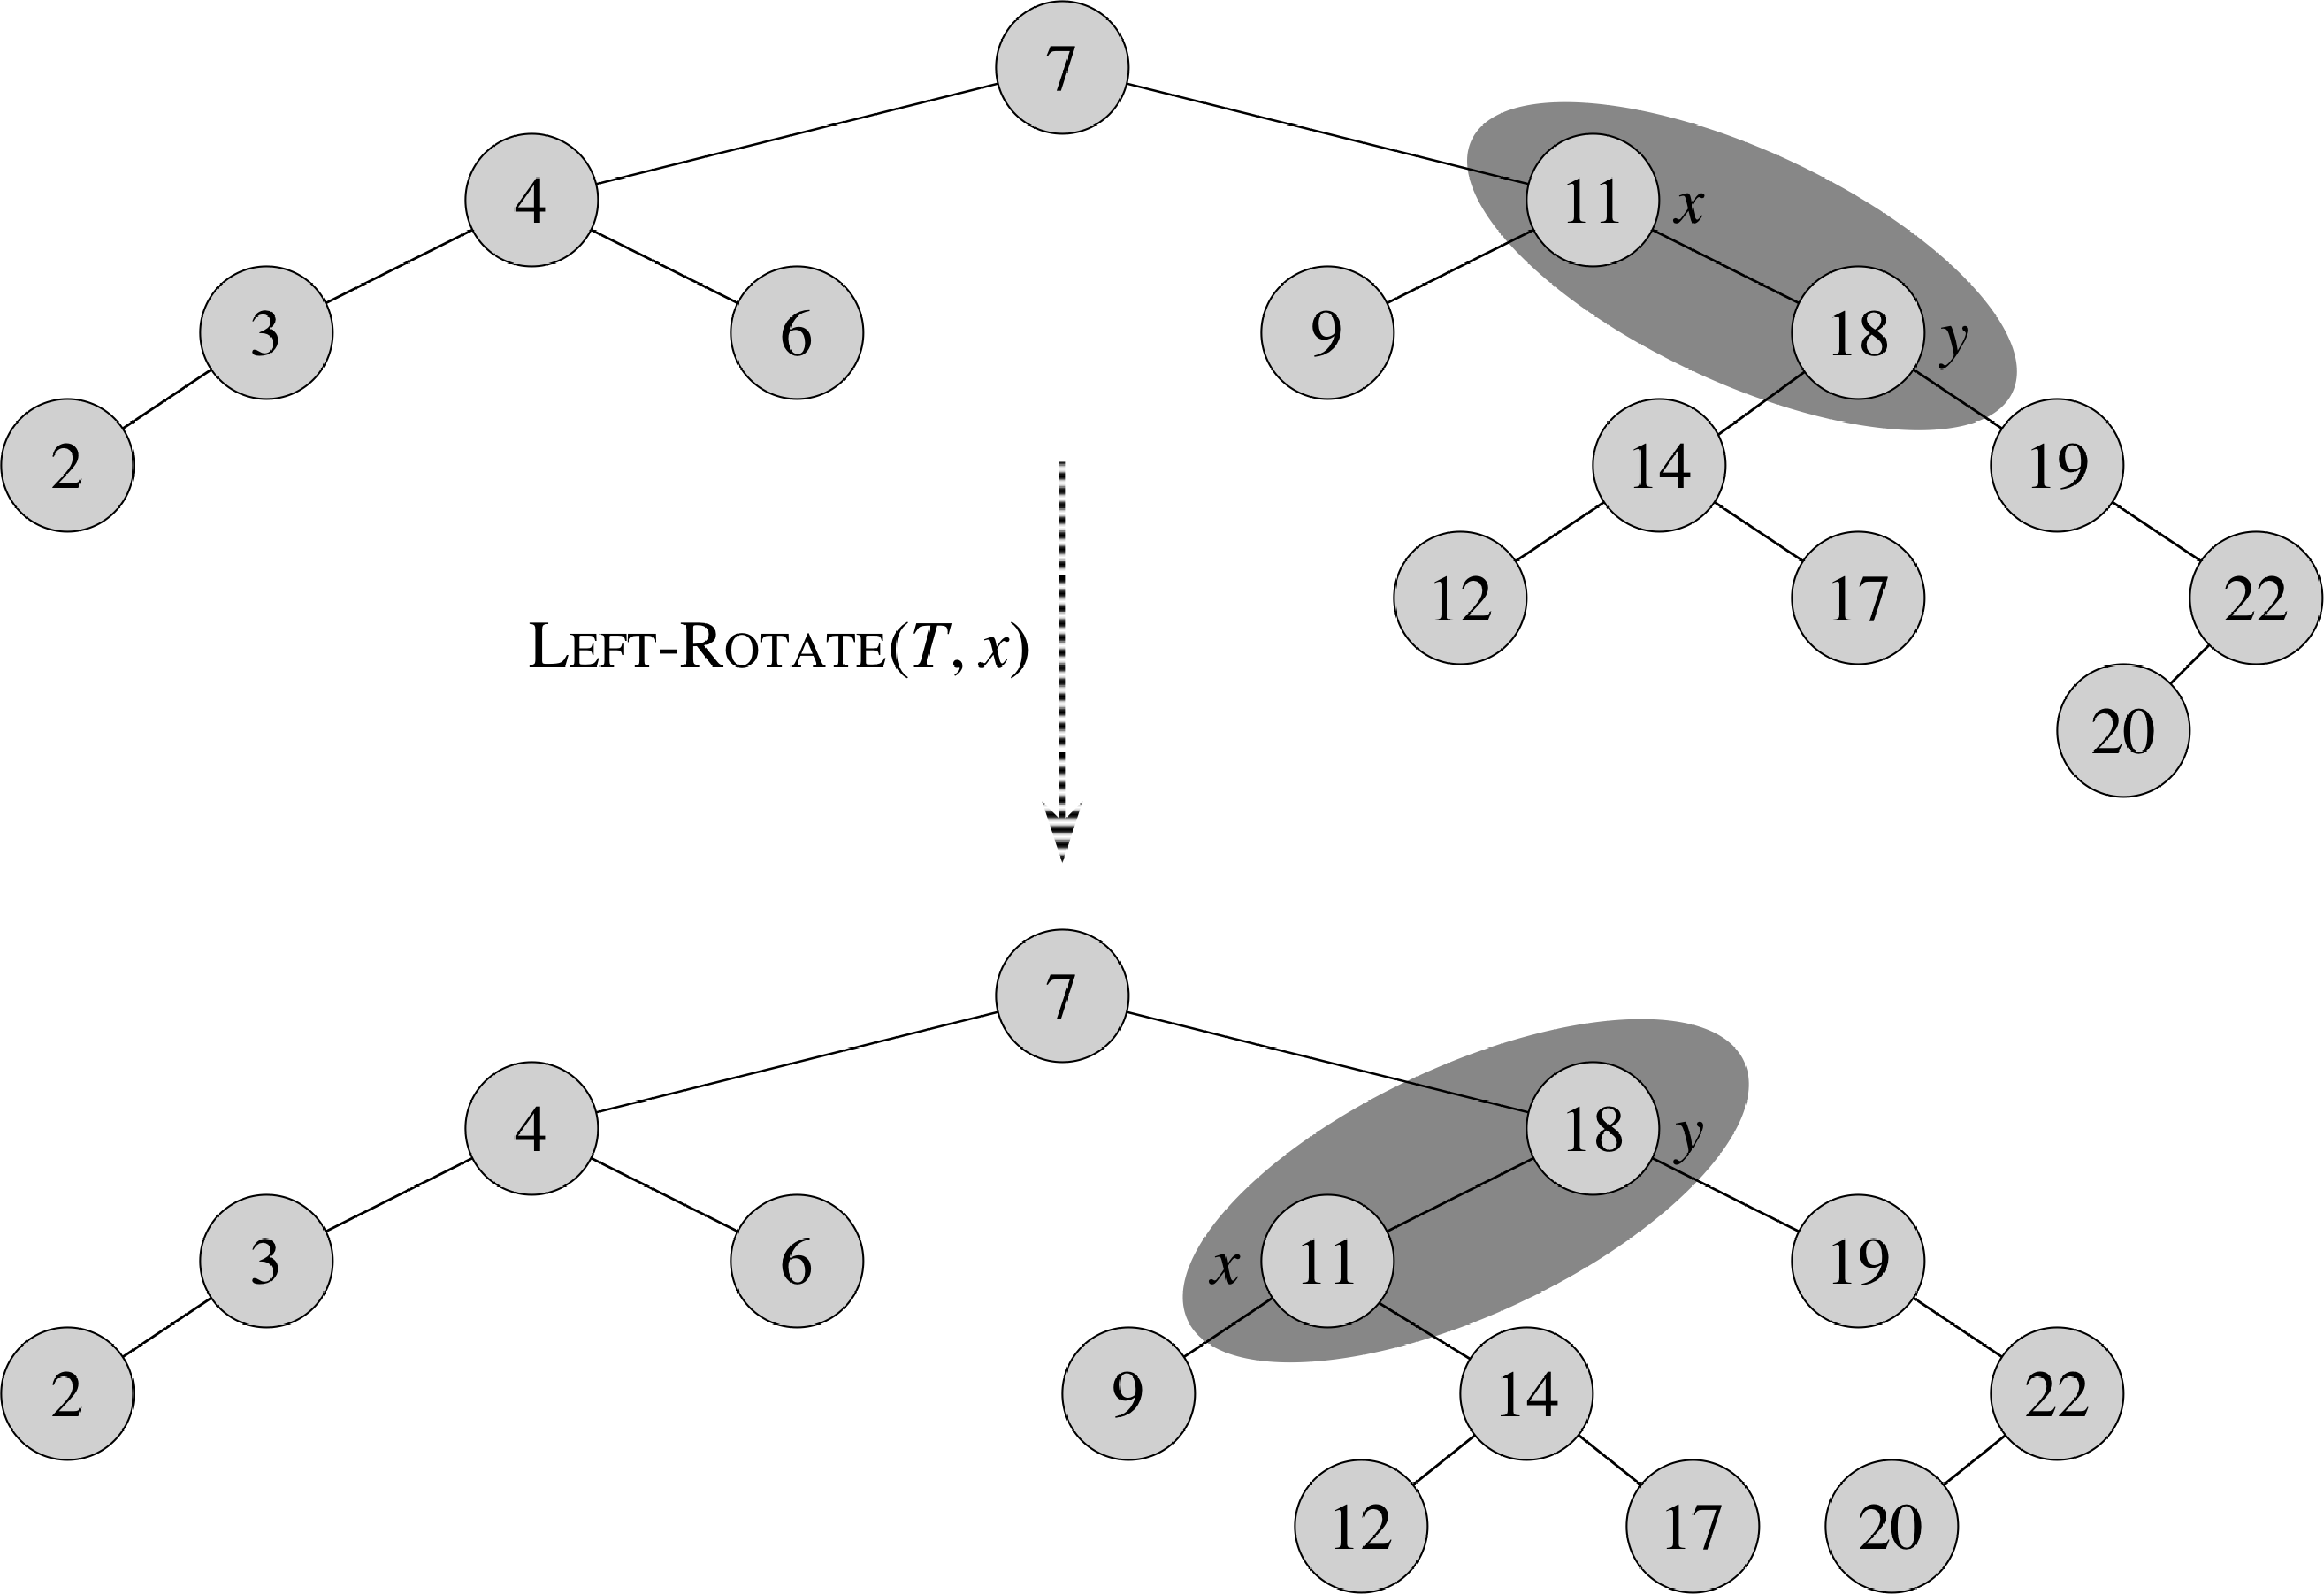
\includegraphics[width=\textwidth]{Fig-13-3.pdf}

\end{frame}

\sect{}
\begin{multicols}{2}
  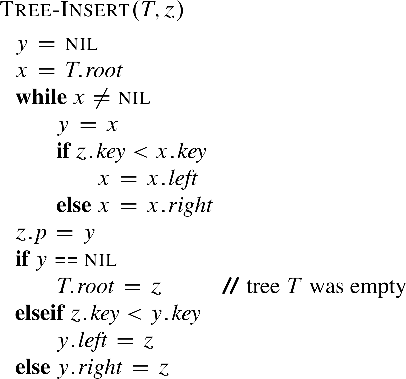
\includegraphics[scale=1]{Tree-Insert}
  \vfill
  \mbox{}
\columnbreak
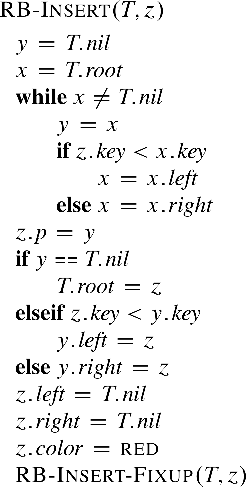
\includegraphics[scale=1]{RB-Insert}
\end{multicols}
\end{frame}

\sect{Insertion fixup}
%\scriptsize
%\begin{multicols}{2}
\bi
\ii Start by doing regular binary-tree insertion.
\ii Color new node red.
\ii May violate red-black tree properties 2 or 4:
\ei

\begin{enumerate}
  \ii Every node is either red or black.

  OK.
  \ii The root is black.

  New node might be root.
  \ii Every leaf ($\attrib{T}{nil}$) is black.

   OK.
  \ii If a node is red, then both its children are black.
  
  New node's parent might be red.
  \ii For each node, all paths from the node to descendant leaves
  contain the same number of black nodes.

  OK.
\end{enumerate}

%\columnbreak
\end{frame}

\sect{}
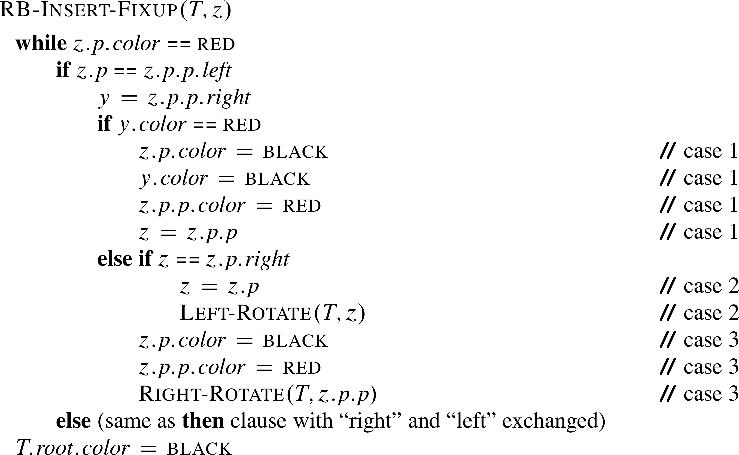
\includegraphics[scale=0.9]{RB-Insert-Fixup}
%\end{multicols}
\end{frame}

\sect{Insertion fixup}
\begin{multicols}{2}
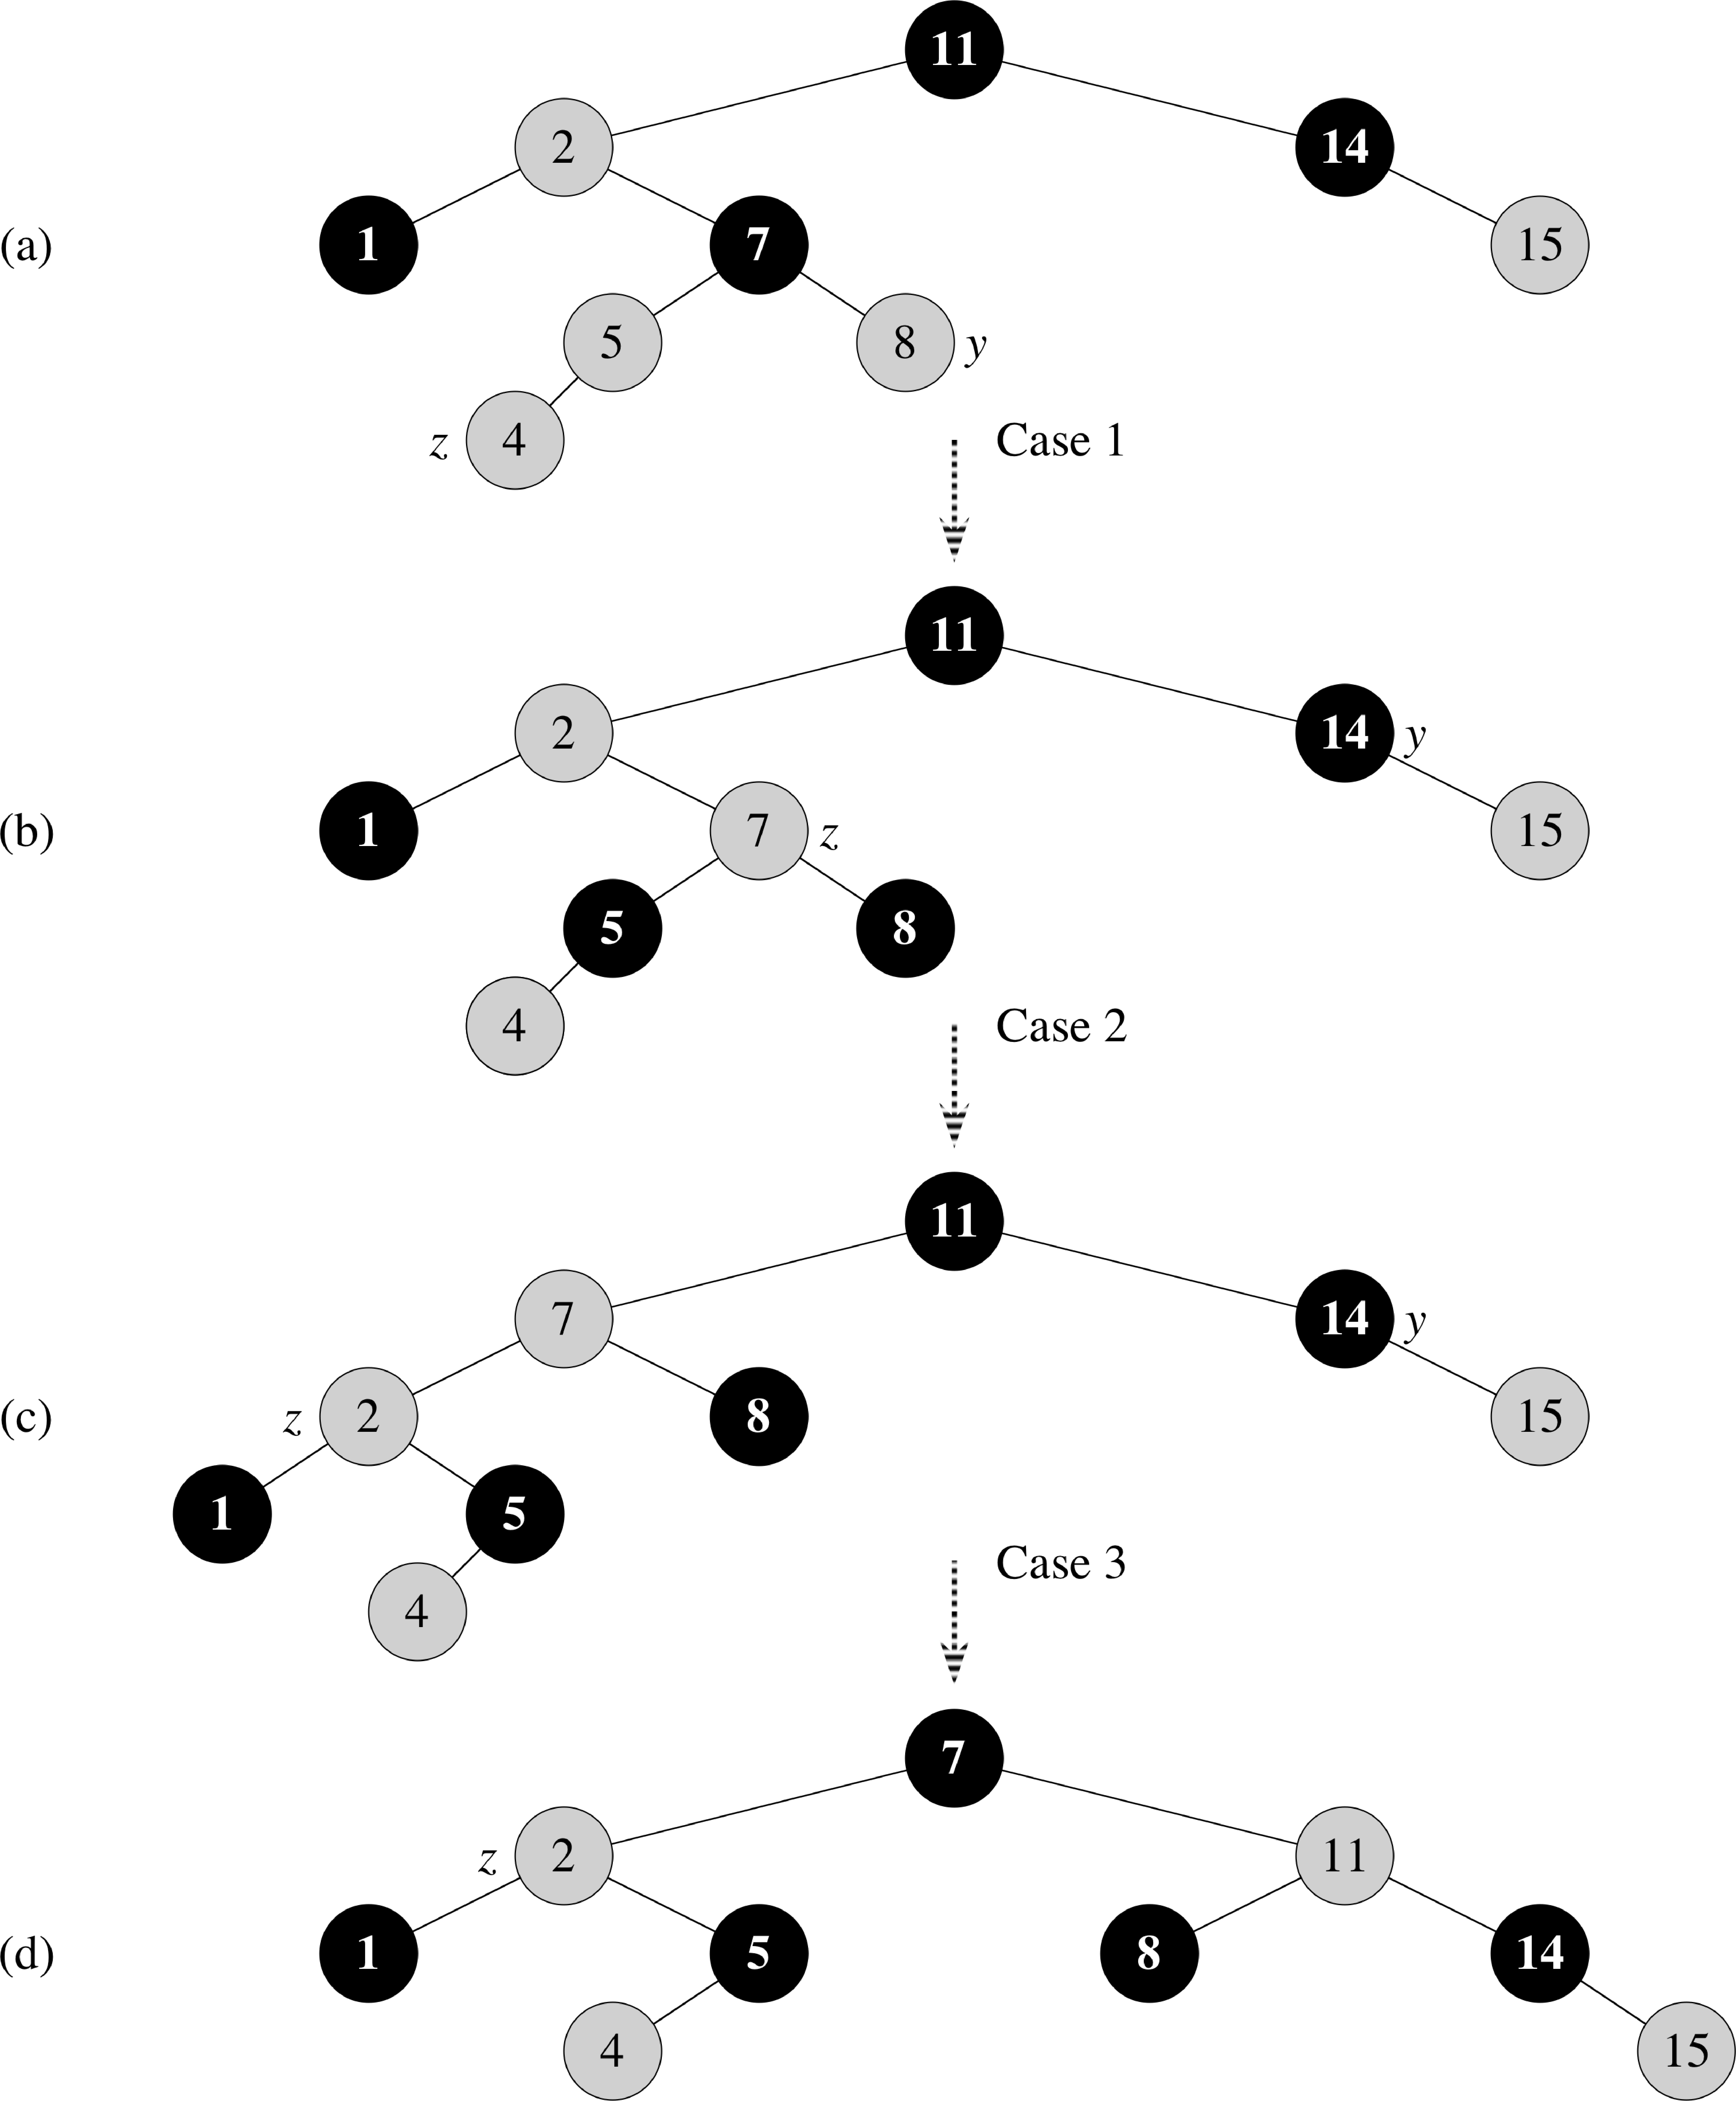
\includegraphics[height=0.8\textheight]{Fig-13-4.pdf}
\columnbreak

  \begin{description}
  \ii Case 1, uncle red:
  \bi
  \ii make gramma's children black
  \ii make gramma red
  \ii make gramma new $z$
  \ii loop
  \ei
\ii Case 2 (optional):
\bi
\ii rotate left
\ei
\ii Case 3:
\bi
\ii rotate right
\ii make parent black
\ei
  \end{description}
\end{multicols}
\end{frame}

\newcommand{\rbinsertfixup}{
\begin{codebox}
  \Procname{$\proc{RB-Insert-Fixup}(T,z)$}
  \li \While $\attrib{\attrib{z}{p}}{color} \isequal \const{red}$\Do
  \li \If $\attrib{z}{p} \isequal
  \attrib{\attrib{\attrib{z}{p}}{p}}{left}$ \Do
  \li $y \gets \attrib{\attrib{\attrib{z}{p}}{p}}{right}$
  \li \If $\attrib{y}{color} \isequal \const{red}$\Do 
  \li $\attrib{\attrib{z}{p}}{color} \gets \const{black}$
%  \RComment{\color{red} case 1}
  \li $\attrib{y}{color}\gets \const{black}$
  \li $\attrib{\attrib{\attrib{z}{p}}{p}}{color} \gets \const{red}$
  \li $z\gets\attrib{\attrib{z}{p}}{p}$
  \li \Else \If $z\isequal\attrib{\attrib{z}{p}}{right}$ \Do
             \li $z\gets\attrib{z}{p}$ %\RComment{ \color{red} case 2}
             \li $\proc{Left-Rotate}(T,z)$ \End
  \li $\attrib{\attrib{z}{p}}{color} \gets \const{black}$
%  \RComment{\color{red} case 3}
  \li $\attrib{\attrib{\attrib{z}{p}}{p}}{color} \gets \const{red}$
  \li $\proc{Right-Rotate}(T,\attrib{\attrib{z}{p}}{p})$
\End
  \li \Else \li (``right'' $\rightleftharpoons$ ``left'') \End
\End
  \li $\attrib{\attrib{T}{root}}{color} \gets \const{black}$
\end{codebox}
}
\sect{}
\begin{multicols}{2}
\footnotesize
\begin{codebox}
  \Procname{$\proc{RB-Insert-Fixup}(T,z)$}
  \li \While $\attrib{\attrib{z}{p}}{color} \isequal \const{red}$\Do
  \li \If $\attrib{z}{p} \isequal
  \attrib{\attrib{\attrib{z}{p}}{p}}{left}$ \Do
  \li $y \gets \attrib{\attrib{\attrib{z}{p}}{p}}{right}$
  \li \If $\attrib{y}{color} \isequal \const{red}$\Do 
  \li $\attrib{\attrib{z}{p}}{color} \gets \const{black}$
%  \RComment{\color{red} case 1}
  \li $\attrib{y}{color}\gets \const{black}$
  \li $\attrib{\attrib{\attrib{z}{p}}{p}}{color} \gets \const{red}$
  \li $z\gets\attrib{\attrib{z}{p}}{p}$
  \li \Else \If $z\isequal\attrib{\attrib{z}{p}}{right}$ \Do
             \li $z\gets\attrib{z}{p}$ %\RComment{ \color{red} case 2}
             \li $\proc{Left-Rotate}(T,z)$ \End
  \li $\attrib{\attrib{z}{p}}{color} \gets \const{black}$
%  \RComment{\color{red} case 3}
  \li $\attrib{\attrib{\attrib{z}{p}}{p}}{color} \gets \const{red}$
  \li $\proc{Right-Rotate}(T,\attrib{\attrib{z}{p}}{p})$
\End
  \li \Else \li (``right'' $\rightleftharpoons$ ``left'') \End
\End
  \li $\attrib{\attrib{T}{root}}{color} \gets \const{black}$
\end{codebox}

  \columnbreak
  
Loop Invariant:  at the start of each iteration of the {\bf while} loop:
\bi
\ii $z$ is red
\ii If $z.p$ is the root, then $z.p$ is black.
\ii There is at most one red-black violation:
\bi
\ii $z$ is a red root.
\ii $z$ and $\attrib{z}{p}$ are both red.
\ei
\ei
\end{multicols}
\end{frame}

\sect{Loop invariant}



Loop Invariant:  at the start of each iteration of the {\bf while} loop:
\begin{enumerate}
\ii $z$ is red\label{zisred}
\ii If $z.p$ is the root, then $z.p$ is black.\label{parentisblack}
\ii There is at most one red-black violation:\label{redblack}
\begin{enumerate}
\ii $z$ is a red root.\label{redroot}
\ii $z$ and $\attrib{z}{p}$ are both red.\label{redred}
\end{enumerate}
\end{enumerate}

\begin{description}
\item[Initialization:]
  \bi
  \ii \ref{zisred} because we set it that way.
  \ii \ref{parentisblack} because it was root to begin with.
  \ii \ref{redblack}.\ref{redroot} possible if $z$ is new root.
  \ii \ref{redblack}.\ref{redred} possible if $z.p$ was red.
  \ei
\item[Termination:] 
  \bi
  \ii \ref{redblack}.\ref{redroot} last line fixes red root.
  \ii \ref{redblack}.\ref{redred} loop only terminates when $z.p$ is black.
  \ei 
\end{description}

\end{frame}

\sect{Maintenance, Case 1, uncle is red}

Loop Invariant:  at the start of each iteration of the {\bf while} loop:
\begin{enumerate}
\ii $z$ is red\label{zisred}
\ii If $z.p$ is the root, then $z.p$ is black.\label{parentisblack}
\ii There is at most one red-black violation:\label{redblack}
\begin{enumerate}
\ii $z$ is a red root.\label{redroot}
\ii $z$ and $\attrib{z}{p}$ are both red.\label{redred}
\end{enumerate}
\end{enumerate}

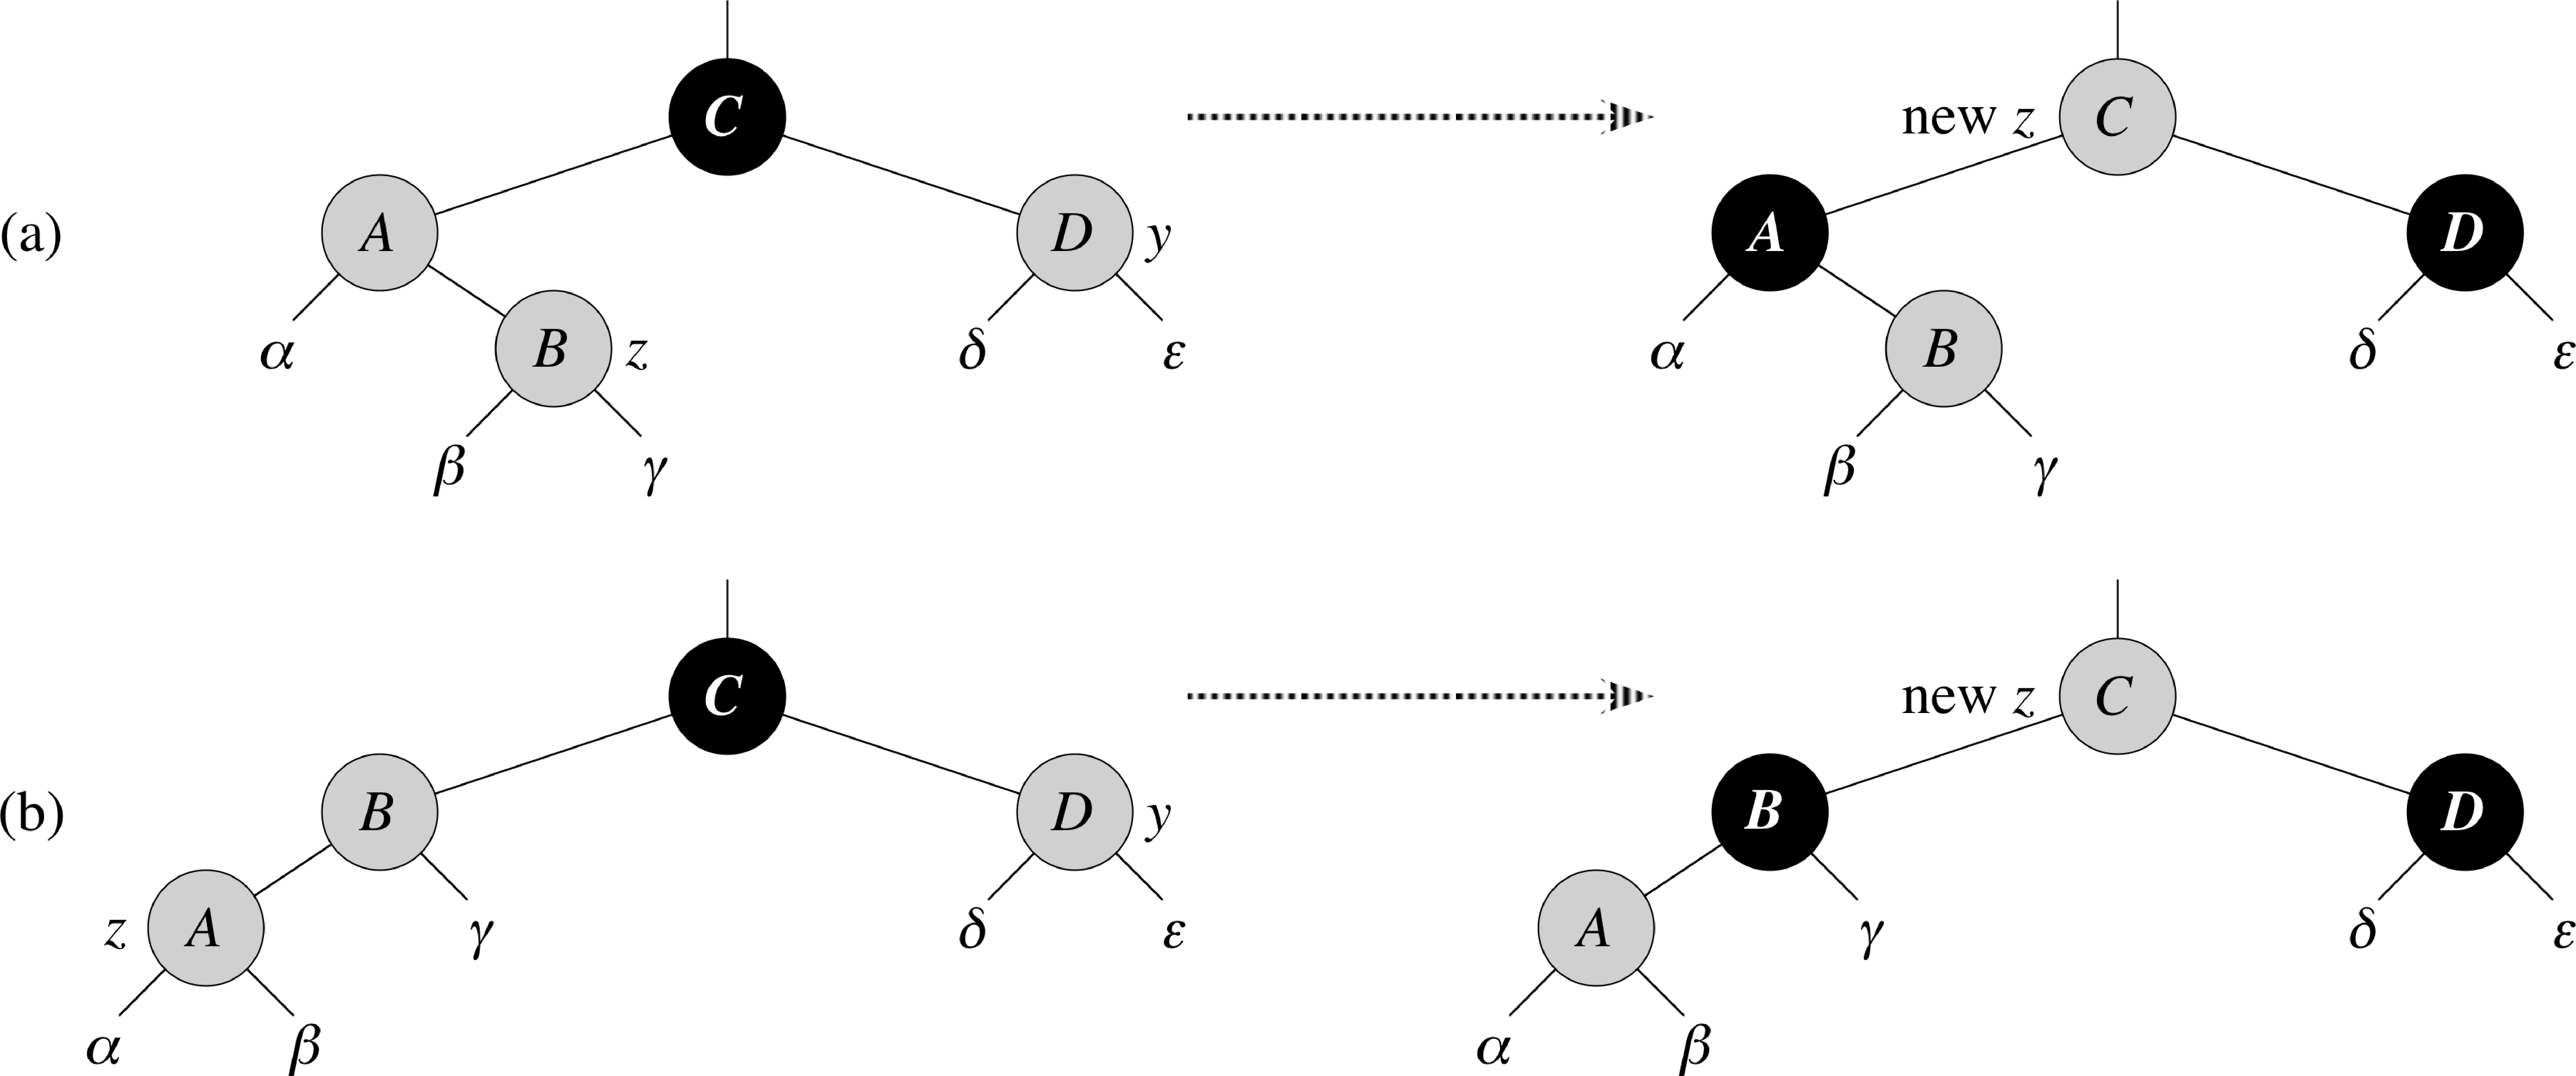
\includegraphics[width=\textwidth]{Fig-13-5.pdf}

\end{frame}

\sect{Maintenance, Case 2\&3, uncle is black:}

Loop Invariant:  at the start of each iteration of the {\bf while} loop:
\begin{enumerate}
\ii $z$ is red\label{zisred}
\ii If $z.p$ is the root, then $z.p$ is black.\label{parentisblack}
\ii There is at most one red-black violation:\label{redblack}
\begin{enumerate}
\ii $z$ is a red root.\label{redroot}
\ii $z$ and $\attrib{z}{p}$ are both red.\label{redred}
\end{enumerate}
\end{enumerate}

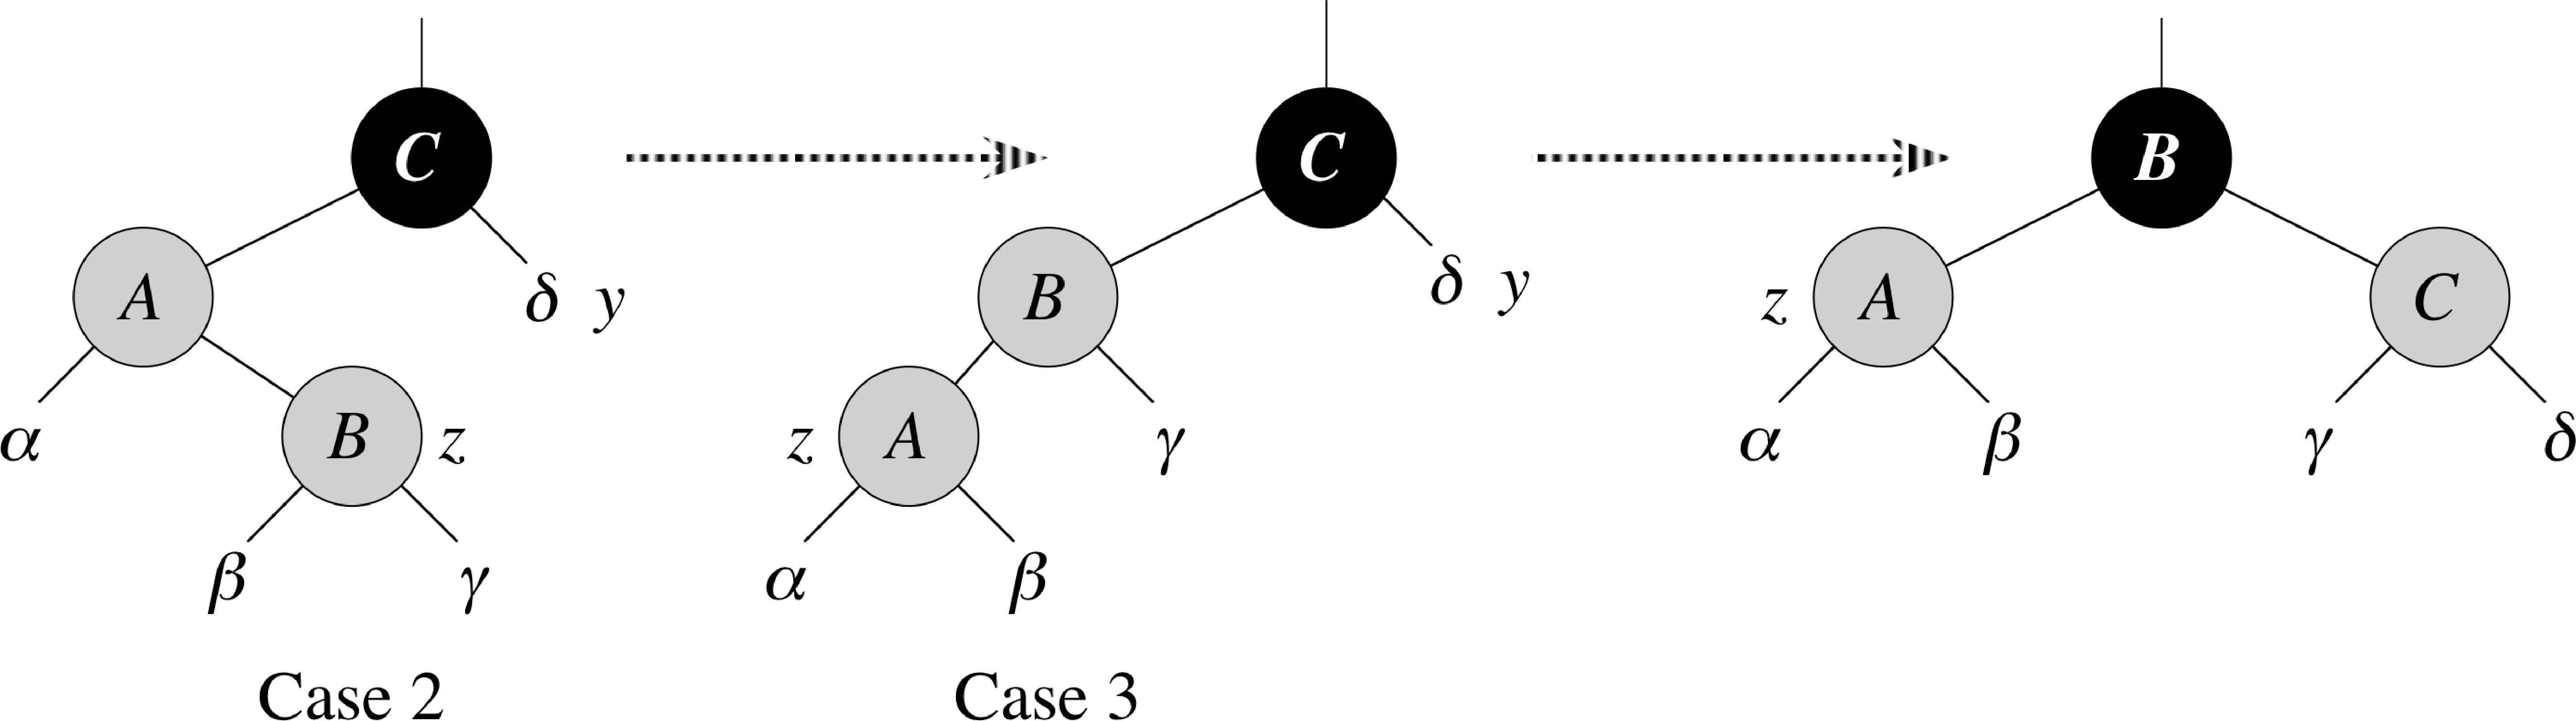
\includegraphics[width=\textwidth]{Fig-13-6.pdf}

\end{frame}

\sect{Analysis}
\bi
\ii $O(\lg n)$ time to insert into binary tree.
\ii Fixup also $O(\lg n)$:
\bi
\ii Each pass through the loop takes $O(1)$ time.
\ii Each iteration moves $z$ up two levels or stops.
\ii $O(\lg n)$ levels.
\ii Also note that there are at most 2 rotations overall.
\ei
\ii Insertion into red-black tree is $O(\lg n)$.
\ei

\end{frame}

\sect{\sc RB-Transplant}

\begin{multicols}{2}
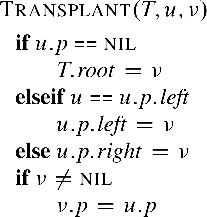
\includegraphics{Transplant}

\columnbreak
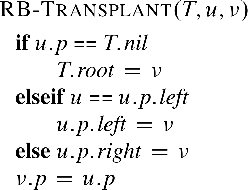
\includegraphics{RB-Transplant}

\end{multicols}

\end{frame}

\sect{}
\scriptsize
\begin{multicols}{2}

  
\begin{codebox}
  \Procname{$\proc{Tree-Delete}(T,z)$}
  \li\If $\attrib{z}{left}\isequal\const{nil}$  \Do
  \li $\proc{Transplant}(T,z,\attrib{z}{right})$ 
  \li \ElseIf $\attrib{z}{right} \isequal \const{nil}$ \Do
  \li $\proc{Transplant}(T,z,\attrib{z}{left})$
  \li \Else 
  \li $y\gets \proc{Tree-Minimum}(\attrib{z}{right})$
  \li \If $\attrib{y}{p} \not\isequal z$ \Do
  \li $\proc{Transplant}(T,y,\attrib{y}{right})$
  \li $\attrib{y}{right}\gets\attrib{z}{right}$
  \li $\attrib{\attrib{y}{right}}{p} \gets y$\End
  \li $\proc{Transplant}(T,z,y)$
  \li $\attrib{y}{left}\gets\attrib{z}{left}$
  \li $\attrib{\attrib{y}{left}}{p} \gets y$
  \End
\end{codebox}

Differences:
\bi
\ii $y$ is either $z$ or the node moved
\ii save $y$'s color
\ii $x$ is node that moves into $y$'s original position
\ii set $x.p$ to original position of $y.p$
\bi
\ii in $x.p = y$, or
\ii in {\sc RB-Transplant}
\ei
\ii {\sc RB-Delete-Fixup} if $y$ was black
\ei

\columnbreak

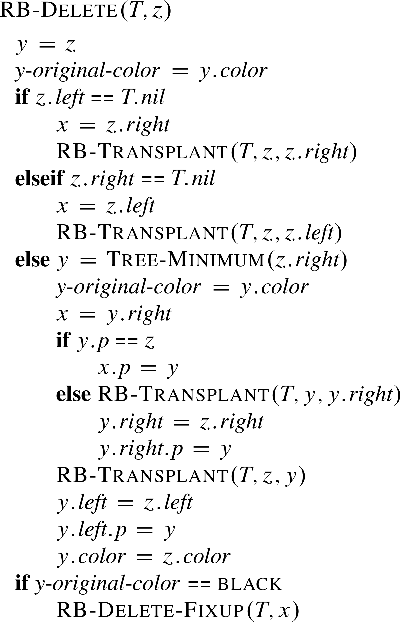
\includegraphics[scale=0.8]{RB-Delete}

\end{multicols}
\end{frame}

\sect{What violations could occur if $y$ was black?}
\begin{enumerate}
  \ii Every node is either red or black.
Still  OK.
  \ii The root is black.

  Violation if $y$ is the root and $x$ is red.
  \ii Every leaf ($\attrib{T}{nil}$) is black.
Still
  OK.

  \ii If a node is red, then both its children are black.

  Violation if $x.p$ and $x$ are both red.
  \ii All paths from a node to descendent leaves
  have same number of black nodes.

  Any paths containing $y$ now have 1 fewer black.

  \bi
  \ii Correct by giving $x$ an ``extra black.''
  \ii Add 1 to count of black nodes on paths containing $x$.
  \ii Now 5 is OK, but 1 is not.
  \ii $x$ is either {\bf black\&black} or {\bf red\&black}
  \ii $x.color$ is still either {\sc red} or {\sc black}
  \ii $x$ just marks the node with a black to move somewhere.
  \ei
\end{enumerate}
\end{frame}

\sect{\sc RB-Delete-Fixup}
\bi
\ii Idea: move the extra black up the tree until
\bi
\ii $x$ points to a {\bf red\&black} node $\implies$ turn it black,
\ii $x$ points to the root $\implies$ just remove the extra black, or
\ii we can do rotations and recolorings to finish.
\ei
\ii Within the {\bf while} loop:
\bi
\ii $x$ always points to a nonroot doubly black node
\ii $w$ is $x$'s sibling
\ii $w$ cannot be $T.nil$ since that would violate 5 at $x.p$.
\ei
\ii Four cases when $x$ is a left child:
\bi
\ii Case 1: $w$ is red
\ii Case 2: $w$'s children both black
\ii Case 3: $w$'s left child red, right child black
\ii Case 4: $x$'s right child red
\ei
\ei
\end{frame}

\sect{}
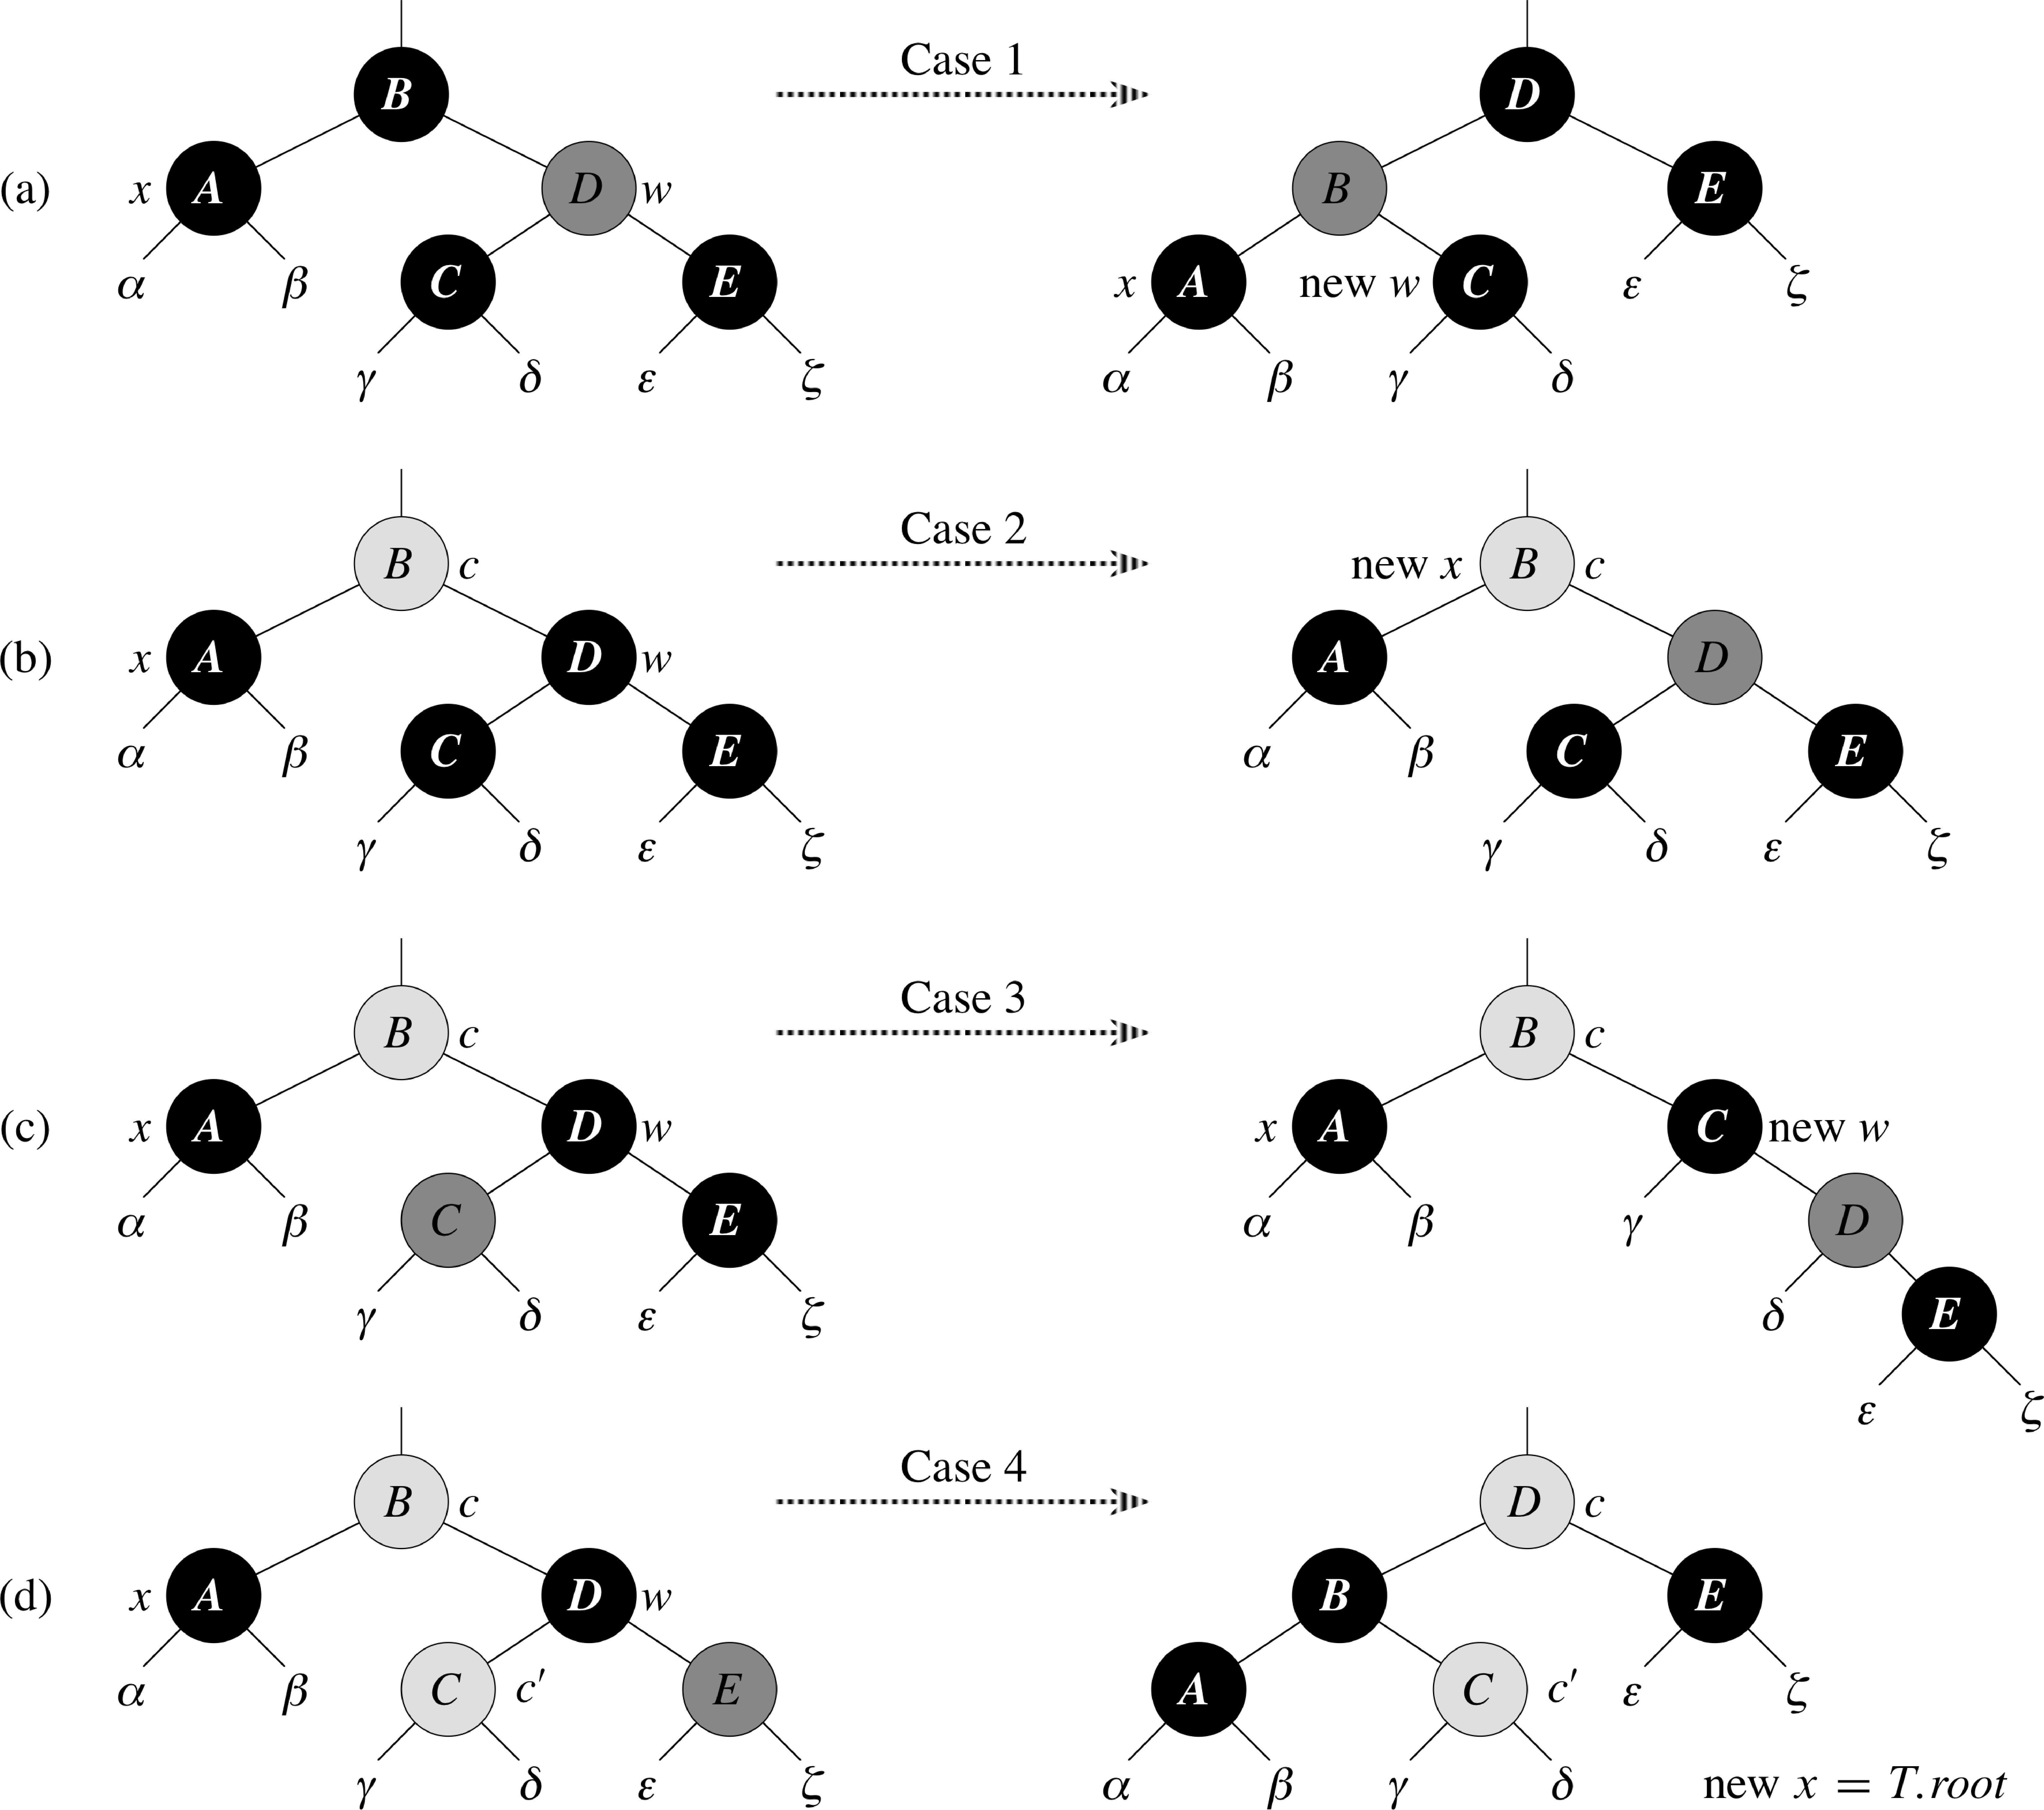
\includegraphics[height=0.9\textheight]{Fig-13-7.pdf}
\end{frame}

\sect{}
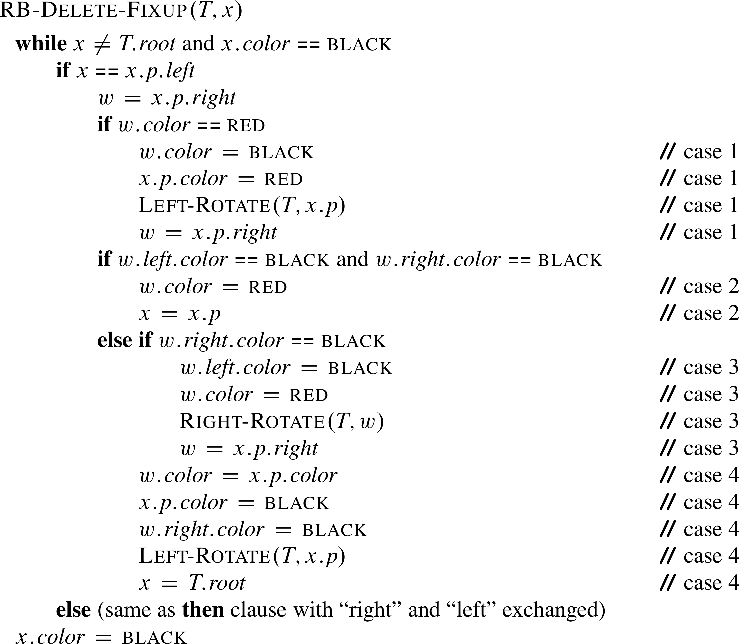
\includegraphics[scale=0.8]{RB-Delete-Fixup}
\end{frame}

\sect{Analysis}
\bi
\ii $O(\lg n)$ time for {\sc RB-Delete} up to the call
of {\sc RB-Delete-Fixup}
\ii Within {\sc RB-Delete-Fixup}:
\bi
\ii Case 2 is the only case in which more iterations occur:
\bi
\ii $x$ moves up 1 level
\ii Hence $O(\lg n)$ iterations
\ei
\ii Each of cases 1, 3, and 4 has 1 rotation $\implies$
$\leq 3$ rotations in all
\ii Hence, $O(\lg n)$ time.
\ei
\ii Note:
\ii Red-black trees use at most a constant number of rotations.
\ii AVL trees in worst case use $\Omega(\lg n)$ rotations.
\ei
\end{frame}

%\sect{}
%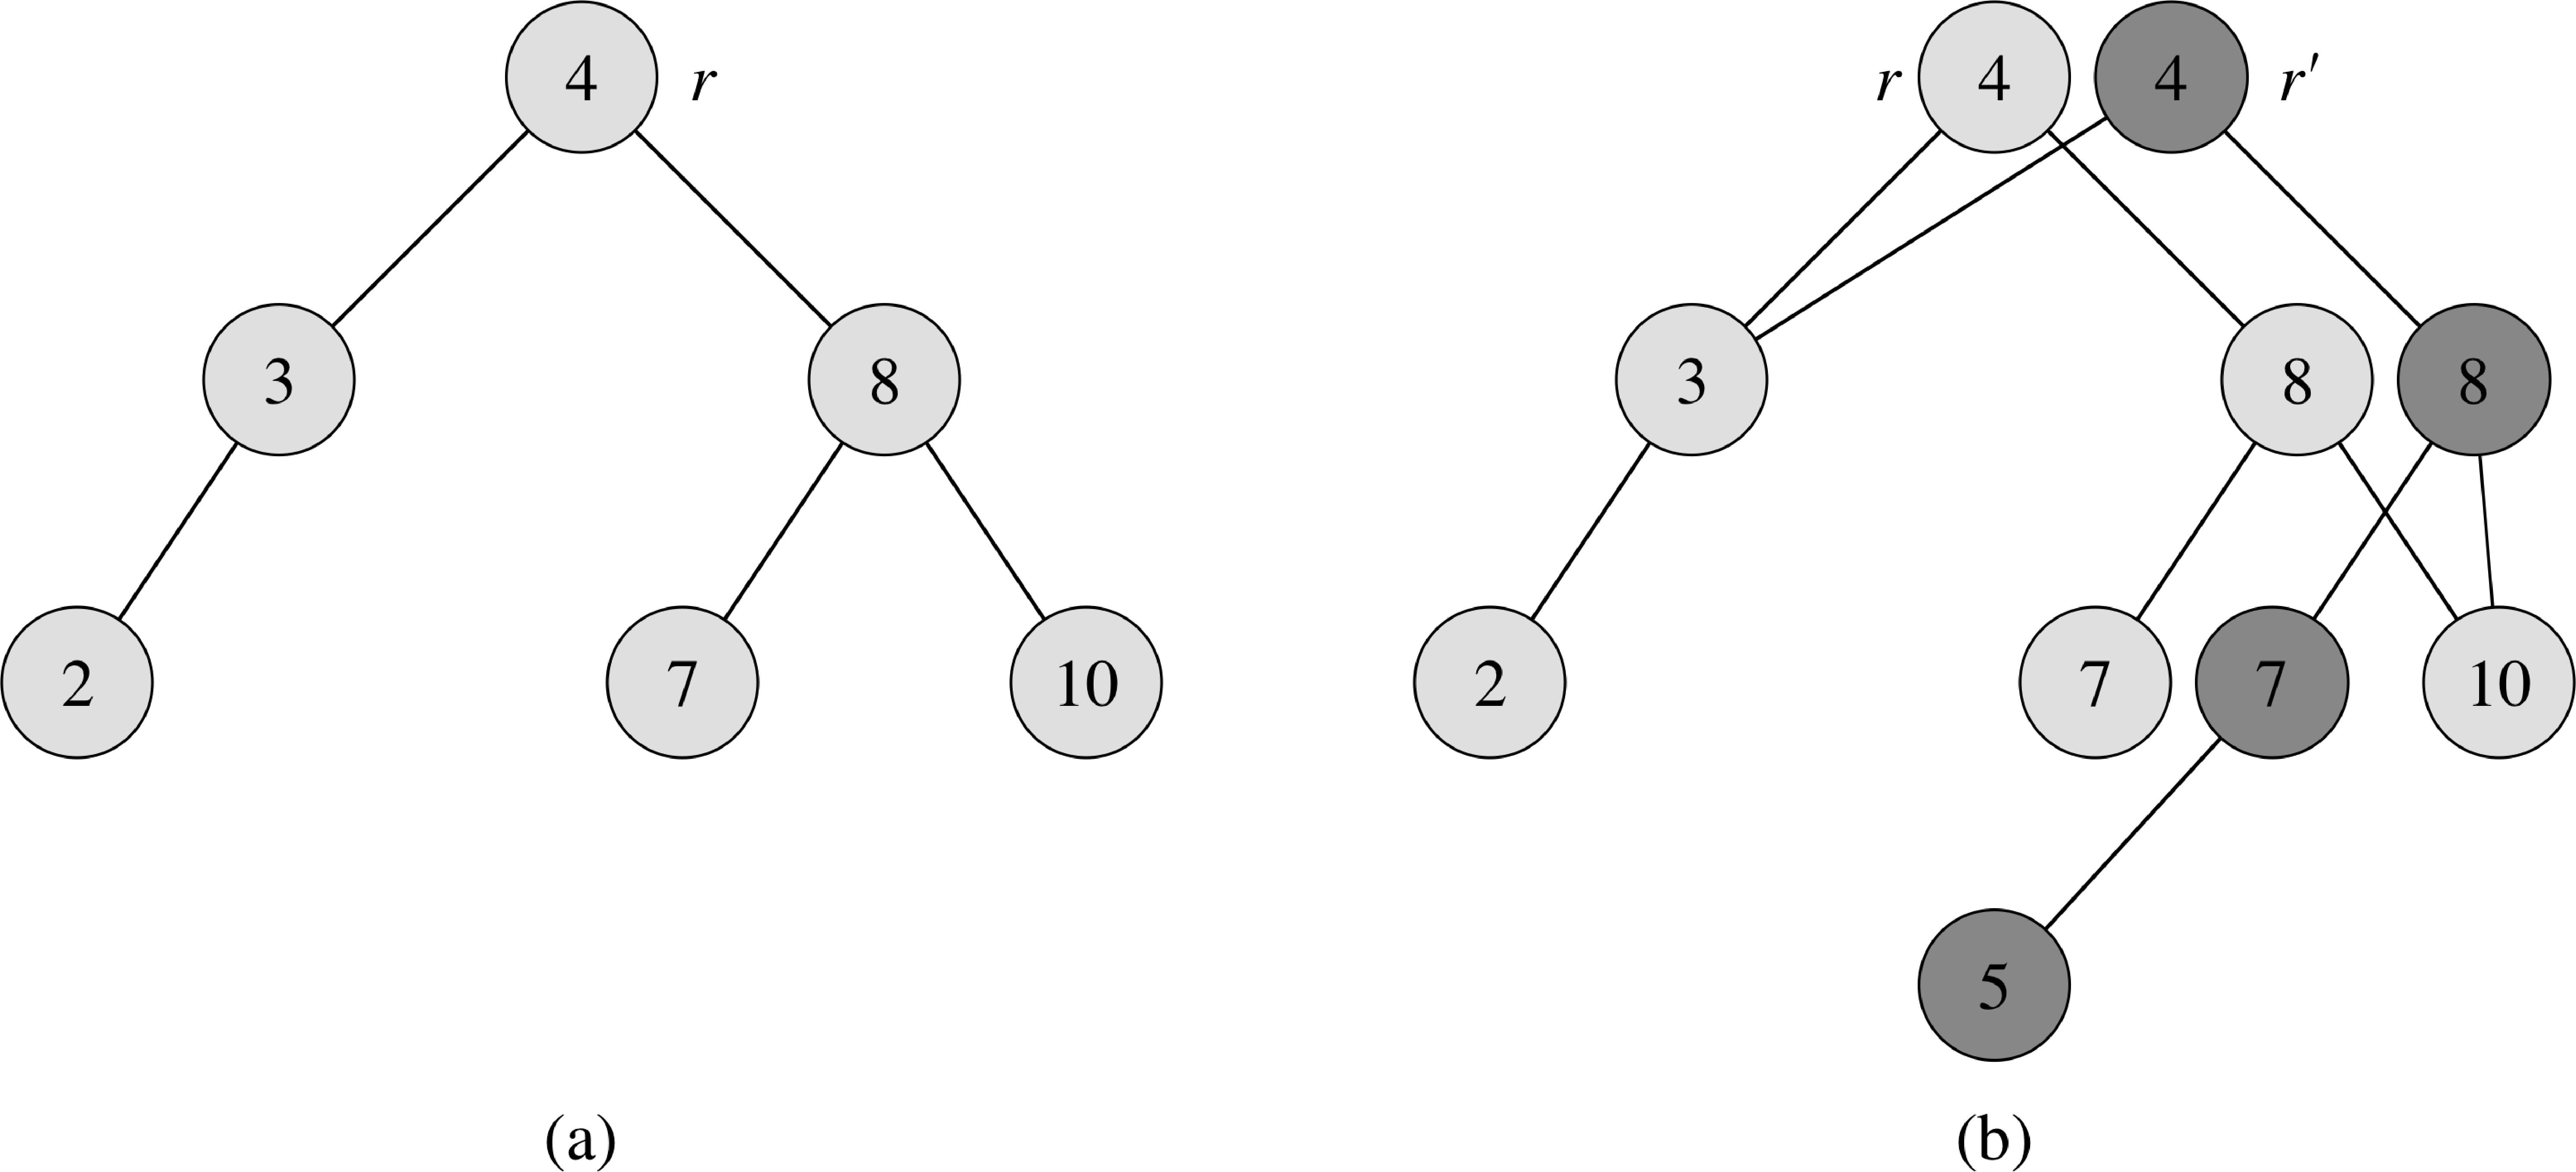
\includegraphics[width=\textwidth]{Fig-13-8.pdf}
%\end{frame}
%\sect{}
%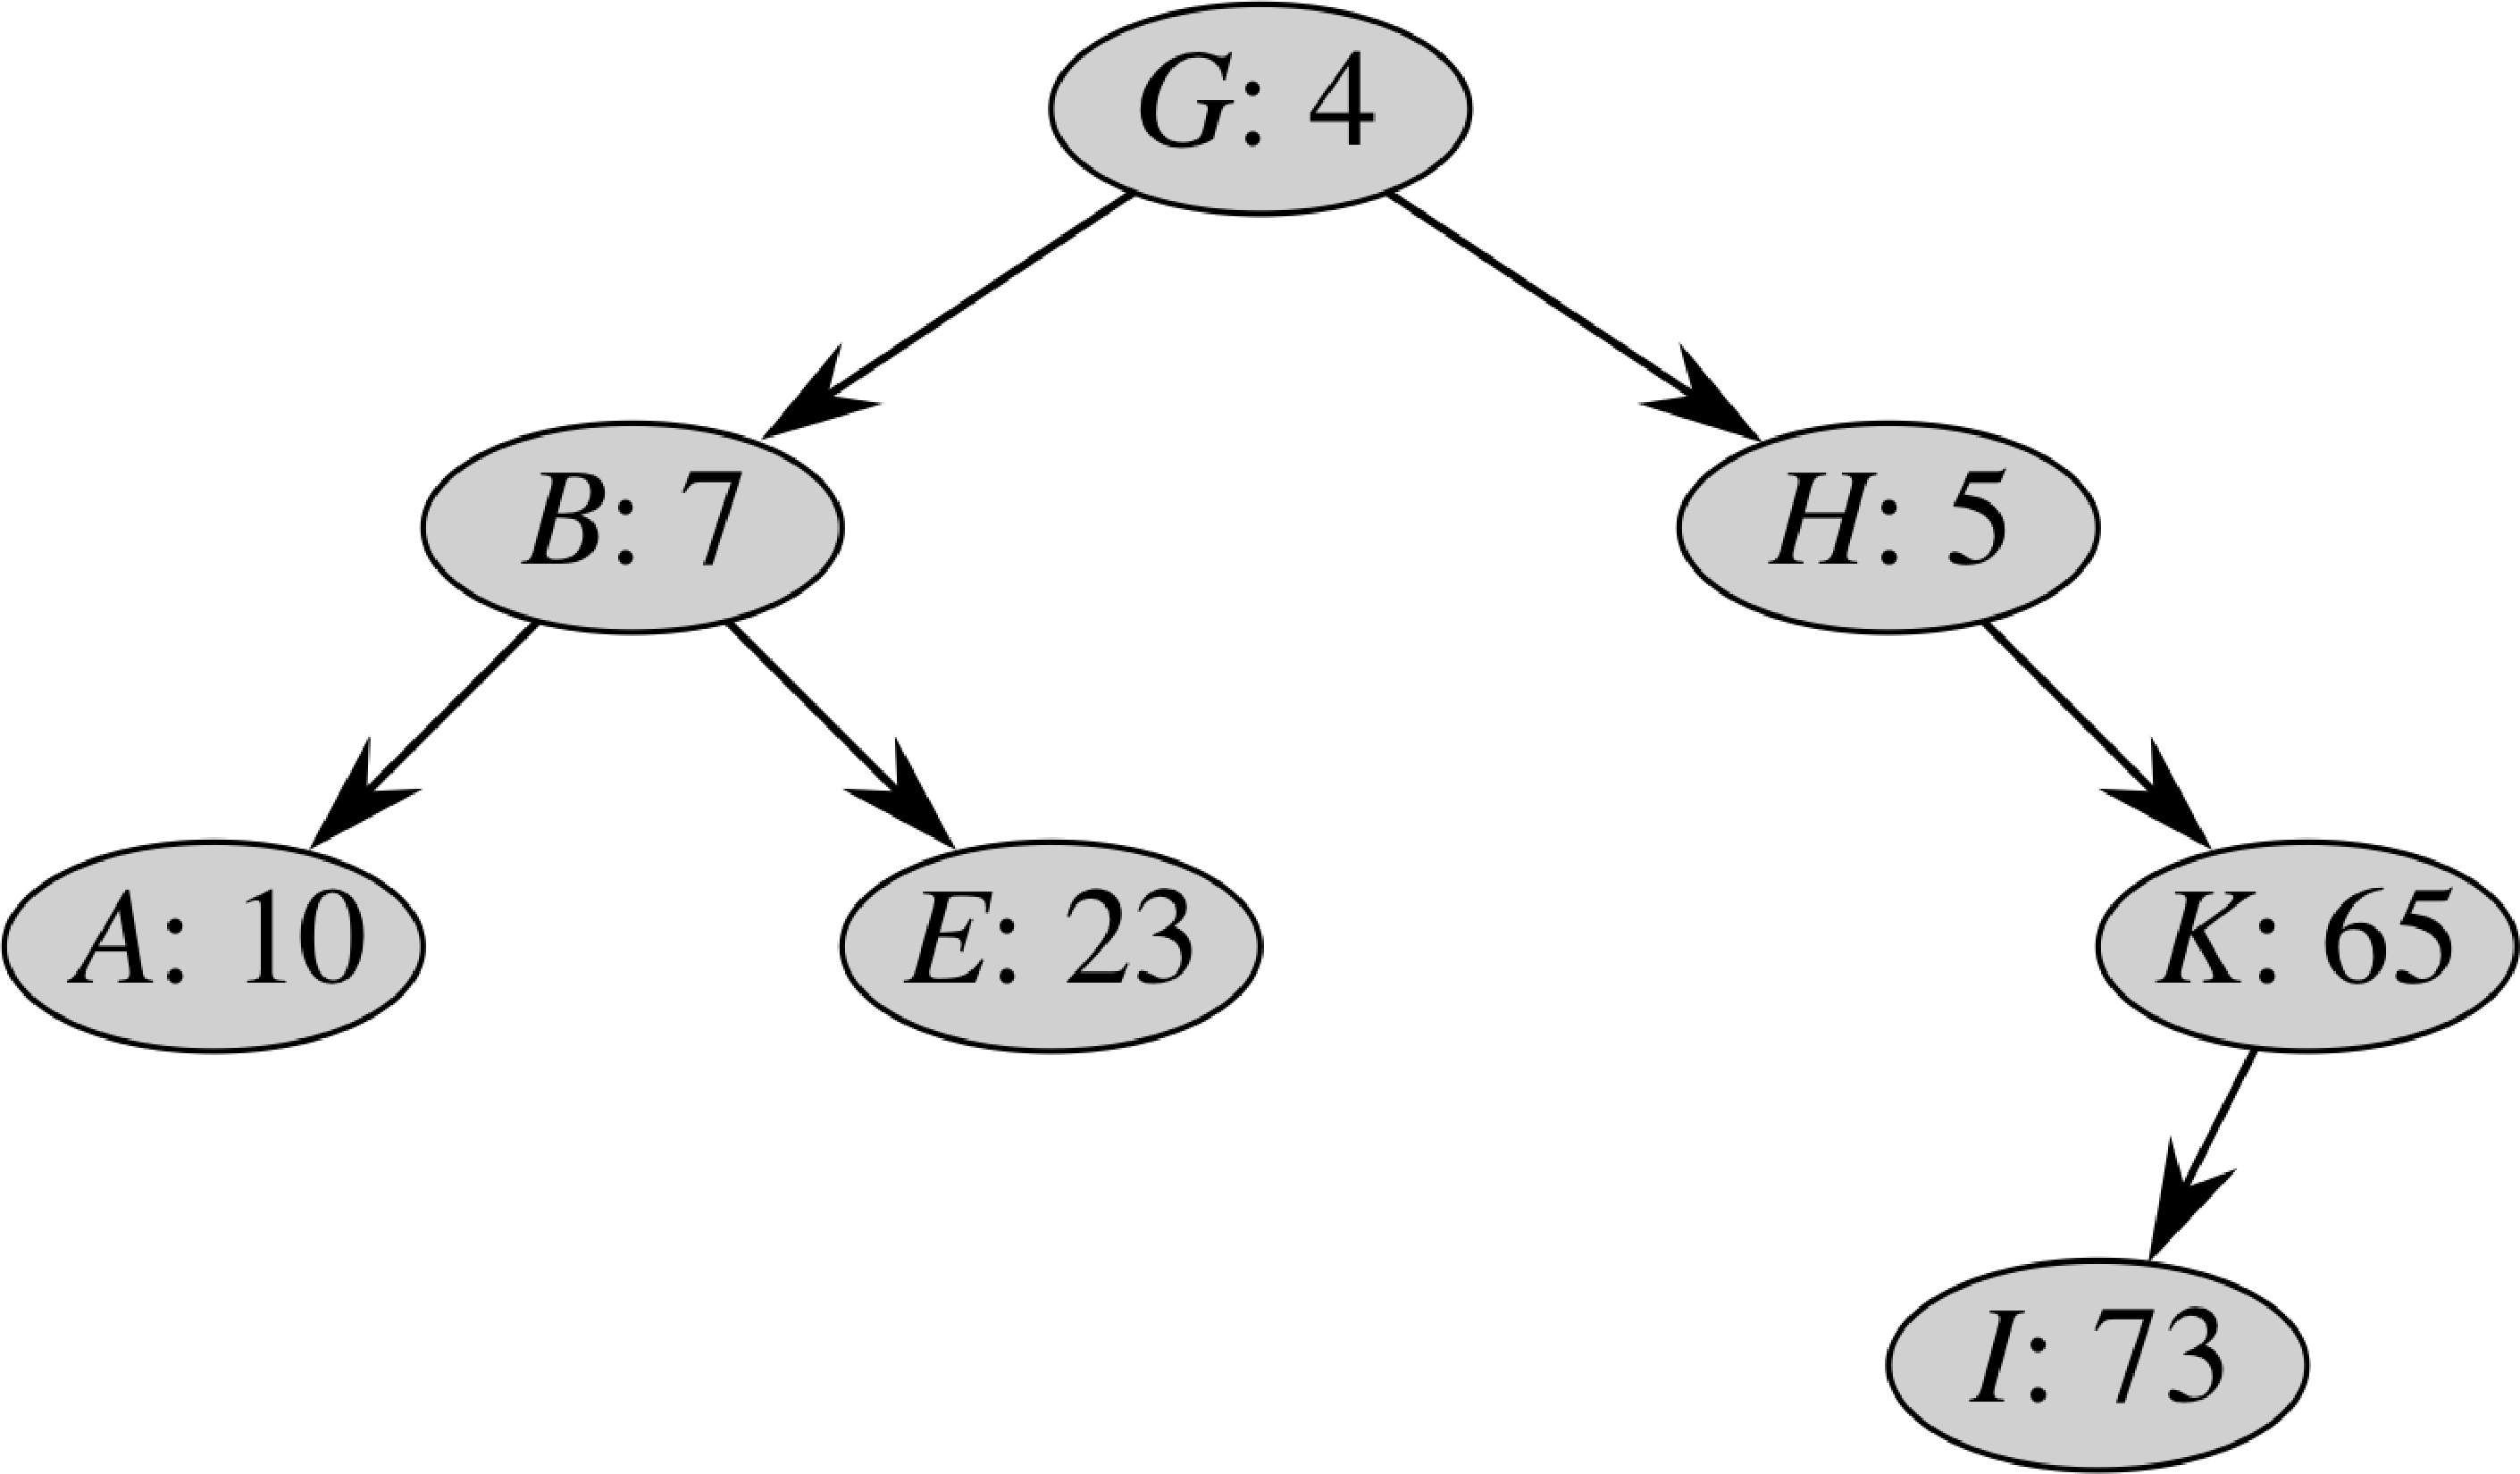
\includegraphics[width=\textwidth]{Fig-13-9.pdf}
%\end{frame}


\end{document}
